% AI for Educators: Part A (non-tech core, ai_core_nontech_*) + Part B (education material).
% Pattern for every AI-for-X seminar: core first, then the audience part, then wrap-up. See AI_FOR_X_PLAN.md.
% Size: 16 core frames + Part B (see ../AI_FOR_X_PLAN.md). To shorten, comment frames in place (do not delete them).

\section[Core]{AI Basics}
% Part A (non-tech core) of the AI-for-X seminars: what AI and generative AI are. 4 frames.
% Adapted from ai_educators_content.tex (Big Picture, Language Model, Large). Audience-neutral on purpose.
% Part A is shared: edit here, then recompile every deck that includes it. Trim by commenting frames, not deleting.
% Size target: same as ai_core_tech_whatisai (4 frames).

%%%%%%%%%%%%%%%%%%%%%%%%%%%%%%%%%%%%%%%%%%%%%%%%%%%%%%%%%%%
\begin{frame}[fragile]\frametitle{The Big Picture: AI, ML, and Deep Learning}
\begin{center}
\includegraphics[width=0.55\linewidth,keepaspectratio]{ai1}
\end{center}
\begin{itemize}
\item \textbf{AI}: any machine doing something that looks intelligent
\item \textbf{Machine Learning (ML)}: a machine that learns the pattern from data, instead of being told the rule directly
\item \textbf{Deep Learning (DL)}: ML using many-layered neural networks, powerful enough to learn something as complex as language
\end{itemize}
{\tiny (Ref: https://blogs.nvidia.com/blog/2016/07/29/whats-difference-artificial-intelligence-machine-learning-deep-learning-ai/)}
\end{frame}

%%%%%%%%%%%%%%%%%%%%%%%%%%%%%%%%%%%%%%%%%%%%%%%%%%%%%%%%%%%
\begin{frame}[fragile]\frametitle{What Is a Language Model?}
\begin{itemize}
\item While typing an SMS, have you noticed it suggests the next word?
\item Those suggestions are not random: the phone has learned what word usually comes next from millions of past sentences.
\item Do this once, word by word, and you get a suggestion. Do it again and again, and you get a full sentence.
\item That is a \textbf{Language Model}, predicting the next word. Chained together, it writes whole paragraphs: a \textbf{Generative Model}.
\end{itemize}
\begin{center}
\includegraphics[width=0.4\linewidth,keepaspectratio]{chatgpt34}
\end{center}
\end{frame}

%%%%%%%%%%%%%%%%%%%%%%%%%%%%%%%%%%%%%%%%%%%%%%%%%%%%%%%%%%%
\begin{frame}[fragile]\frametitle{Why Are They Called ``Large''?}
\begin{itemize}
\item ChatGPT works on exactly this idea, just at an enormous scale: trained on a large fraction of everything ever written on the internet.
\item That is why the phrase is \textbf{Large Language Model (LLM)}: large training data, large number of internal parameters.
\item More data and more parameters mean better predictions, but the underlying idea never changes: predict the next word, one at a time.
\end{itemize}
\begin{center}
\includegraphics[width=0.5\linewidth,keepaspectratio]{chatgpt31}
\end{center}
\end{frame}

%%%%%%%%%%%%%%%%%%%%%%%%%%%%%%%%%%%%%%%%%%%%%%%%%%%%%%%%%%%
\begin{frame}[fragile]\frametitle{Generative AI: What It Can Make}
\begin{itemize}
\item \textbf{Generative AI} makes new content from a request: text, images, code, audio, even short video.
\item The chat assistants you may have met (ChatGPT, Claude, Gemini and others) are built on language models like the one on the last slide.
\item Same idea, different material: the model has seen very many examples of the thing, and produces a new one that looks like them.
\item It is a very fast, very well-read assistant. It is not a person, and it does not understand your situation unless you tell it.
\end{itemize}
\end{frame}

% Part A (non-tech core) of the AI-for-X seminars: limits and responsible use. 4 frames.
% Adapted from ai_educators_wrapup.tex (failure modes, data) and ai_intro_nontech.tex. Audience-neutral on purpose.
% Part A is shared: edit here, then recompile every deck that includes it. Trim by commenting frames, not deleting.
% Size target: same as ai_core_tech_limits (4 frames).

%%%%%%%%%%%%%%%%%%%%%%%%%%%%%%%%%%%%%%%%%%%%%%%%%%%%%%%%%%%
\begin{frame}[fragile]\frametitle{It Predicts, It Does Not Know}
\begin{itemize}
\item A language model writes the most likely next words. It does not look facts up, and it does not know when it is wrong.
\item So it can produce a fluent, confident answer that is false: a \textbf{hallucination}. Invented names, dates, quotations and references are the classic cases.
\item The more your question depends on one exact fact, the more you must check the answer.
\end{itemize}
\begin{alertblock}{Rule of Thumb}
Fluent does not mean true. Check every fact, name and reference before you rely on it.
\end{alertblock}
\end{frame}

%%%%%%%%%%%%%%%%%%%%%%%%%%%%%%%%%%%%%%%%%%%%%%%%%%%%%%%%%%%
\begin{frame}[fragile]\frametitle{Other Limits Worth Knowing}
\begin{itemize}
\item \textbf{Out of date:} the model learned from text up to some date. Recent events need a web search or a source you supply.
\item \textbf{Bias:} models trained on internet-scale text inherit internet-scale biases. Read the output with that in mind.
\item \textbf{Inconsistency:} ask the same question twice and the answers can differ. Do not treat one answer as a ruling.
\item \textbf{Over-reliance:} a first draft is easy to accept as the final answer. It is a starting point, not a verdict.
\end{itemize}
\end{frame}

%%%%%%%%%%%%%%%%%%%%%%%%%%%%%%%%%%%%%%%%%%%%%%%%%%%%%%%%%%%
\begin{frame}[fragile]\frametitle{What Not to Paste}
\begin{itemize}
\item Public AI tools may keep what you type, and may use it to improve their models, depending on the tool and its settings.
\item \textbf{Never paste} personal data, passwords, contracts, unpublished work or anything confidential into a public AI tool.
\item If you need help with sensitive text, remove the names and details first, or use a tool your organisation has approved.
\end{itemize}
\begin{alertblock}{Rule of Thumb}
If you would not leave it on a sticky note on a public desk, do not paste it into a public AI chat.
\end{alertblock}
\end{frame}

%%%%%%%%%%%%%%%%%%%%%%%%%%%%%%%%%%%%%%%%%%%%%%%%%%%%%%%%%%%
\begin{frame}[fragile]\frametitle{Treat the Output as a First Draft}
\begin{itemize}
\item Read it, correct it, and make it yours before it goes anywhere.
\item You are responsible for what you publish, send or submit, whoever or whatever produced the first version.
\item Ask the tool to show its reasoning or sources, then check them yourself.
\item When in doubt, ask a person who knows the subject.
\end{itemize}
\end{frame}


\section[Prompts]{Prompts with CRAFT}
% Part A (non-tech core) of the AI-for-X seminars: prompts and the CRAFT framework. 8 frames.
% Adapted from llm_promptengg_educators.tex (What Is a Prompt, Same Task, CRAFT x5, Takeaways) with neutral
% examples. The Educators deck keeps its own education examples in its Part B.
% Part A is shared: edit here, then recompile every deck that includes it. Trim by commenting frames, not deleting.
% Size target: same as ai_core_tech_prompts (8 frames).

%%%%%%%%%%%%%%%%%%%%%%%%%%%%%%%%%%%%%%%%%%%%%%%%%%%%%%%%%%%
\begin{frame}[fragile]\frametitle{What Is a Prompt?}
\begin{itemize}
\item A \textbf{prompt} is the text you type to the AI: a question, an instruction, or both.
\item The model reads your prompt and continues it, one word at a time, just like the SMS suggestion.
\item So your words steer the answer: more specific text gives a more specific result.
\item A prompt can hold a role for the AI, background, an example, and the text to work on.
\item \textbf{Prompt engineering} is writing prompts that give usable answers.
\end{itemize}
\end{frame}

%%%%%%%%%%%%%%%%%%%%%%%%%%%%%%%%%%%%%%%%%%%%%%%%%%%
\begin{frame}[fragile]\frametitle{Same Task, Different Prompts}
\begin{itemize}
\item Same AI, same topic: a vague prompt gives a generic answer, a specific one gives a usable answer.
\item A chat remembers what came before. Reply to refine the answer instead of starting again.
\end{itemize}
\begin{lstlisting}[language={}]
Vague:      Write a notice about water tank cleaning.

Specific:   Write a notice for a housing society about
            water tank cleaning on Sunday, 6 to 10 am,
            in 80 words, polite tone.

Follow-up:  Make it shorter, and add a contact number
            placeholder.
\end{lstlisting}
\end{frame}

%%%%%%%%%%%%%%%%%%%%%%%%%%%%%%%%%%%%%%%%%%%%%%%%%%%%%%%%%%%
\begin{frame}[fragile]\frametitle{A Framework for Every Prompt: CRAFT}

\begin{center}
\Large \textbf{C R A F T}
\end{center}

\medskip
\begin{itemize}
    \item \textbf{C}ontext, who you are, what the situation is
    \item \textbf{R}ole, who the AI should act as
    \item \textbf{A}ction, exactly what you want it to do
    \item \textbf{F}ewshots, one or two examples of what ``good'' looks like
    \item \textbf{T}weaks, tone, length, format, and what to avoid
\end{itemize}

\medskip
\begin{center}
\textbf{Run through the five letters in your head before you type. That is the whole framework.}
\end{center}

\end{frame}

%%%%%%%%%%%%%%%%%%%%%%%%%%%%%%%%%%%%%%%%%%%%%%%%%%%%%%%%%%%
\begin{frame}[fragile]\frametitle{CRAFT: Context and Role}

\begin{itemize}
    \item \textbf{Context}, without it, the AI is guessing: what the subject is, who the reader is, what has already happened.
    \item \textbf{Role}, telling the AI who to act as changes its whole register: a ``friendly neighbour'' writes differently from a ``formal clerk.''
\end{itemize}

\begin{lstlisting}[language=HTML]
Weak:  Write a notice about water tank cleaning.

CRAFT: You are the secretary of a housing society (Role).
       The tank is cleaned twice a year, and residents
       have complained about short notice before (Context).
\end{lstlisting}

\end{frame}

%%%%%%%%%%%%%%%%%%%%%%%%%%%%%%%%%%%%%%%%%%%%%%%%%%%%%%%%%%%
\begin{frame}[fragile]\frametitle{CRAFT: Action and Fewshots}

\begin{itemize}
    \item \textbf{Action}, one clear instruction. ``Help me with X'' is not an action, ``Write a 3-line notice about X'' is.
    \item \textbf{Fewshots}, show, do not just tell. One example of the style or format you want is worth three sentences of description.
\end{itemize}

\begin{lstlisting}[language=HTML]
Action:   Write a 3-line notice about the tank
          cleaning on Sunday.

Fewshot:  Match this style:
          "Water supply will be off on Monday,
           9 to 12. Please store water in advance."
\end{lstlisting}

\end{frame}

%%%%%%%%%%%%%%%%%%%%%%%%%%%%%%%%%%%%%%%%%%%%%%%%%%%%%%%%%%%
\begin{frame}[fragile]\frametitle{CRAFT: Tweaks}

\begin{itemize}
    \item \textbf{Tweaks} are the small dials that turn a generic answer into a usable one:
    \begin{itemize}
        \item \textbf{Tone}, formal / friendly / encouraging
        \item \textbf{Length}, word count or ``under 5 sentences''
        \item \textbf{Format}, bullet list / table / email / paragraph
        \item \textbf{Constraints}, what to explicitly avoid
    \end{itemize}
    \item Add tweaks last, once Context, Role, Action, and Fewshots already give the AI enough to work with.
\end{itemize}

\begin{lstlisting}[language=HTML]
Tweaks: Keep it under 60 words, friendly tone,
        no exclamation marks.
\end{lstlisting}

\end{frame}

%%%%%%%%%%%%%%%%%%%%%%%%%%%%%%%%%%%%%%%%%%%%%%%%%%%%%%%%%%%
\begin{frame}[fragile]\frametitle{CRAFT, All Together}

\begin{lstlisting}[language=HTML]
You are the secretary of a housing society (R).
The tank is cleaned twice a year, and residents
have complained about short notice before (C).

Write a 3-line notice about the tank cleaning
on Sunday, 6 to 10 am (A).

Match this style: "Water supply will be off on
Monday, 9 to 12. Please store water in advance." (F)

Keep it under 60 words, friendly tone,
no exclamation marks (T).
\end{lstlisting}

\end{frame}

%%%%%%%%%%%%%%%%%%%%%%%%%%%%%%%%%%%%%%%%%%%%%%%%%%%%%%%%%%%
\begin{frame}[fragile]\frametitle{CRAFT: The Takeaways}

\begin{itemize}
    \item Not every prompt needs all five letters spelled out explicitly, but running through them in your head catches what you would otherwise forget.
    \item Save a prompt that works. A small personal library of tested prompts saves more time than any single clever prompt.
    \item \textbf{Always remember:} treat the output as a first draft, review it, and never paste confidential data into a public AI tool.
\end{itemize}

\end{frame}


\section[Educators]{AI for Educators}
\begin{frame}[fragile]\frametitle{}
\begin{center}
{\Large AI for Educators}
\end{center}
\end{frame}

% ai_educators_content.tex now holds the State / TaskvJob / Programs sections (education-specific);
% its generic AI-basics frames are commented there (covered by the core).
% Merged 2026: folds ai_educators_howaiworks/_stateofplay/_taskvsjob/_programstructure
% into one file (they were 4 small standalone files, 15-72 lines each). Section boundaries
% are marked inline with \section so this single \input still produces 4 separate sections
% in the deck, exactly as before the merge.

% [ai-for-x: commented 2026-11-07 | covered by ai_core_nontech_whatisai.tex]
% \section[WhatAI]{What Is AI?}

% %%%%%%%%%%%%%%%%%%%%%%%%%%%%%%%%%%%%%%%%%%%%%%%%%%%%%%%%%%%
% % [upgrade-deck: moved 2026-10-24 | reorder | AI/ML/DL big picture now opens the deck; same move in ai_educators_content_short.tex]
% \begin{frame}[fragile]\frametitle{The Big Picture: AI, ML, and Deep Learning}
% \begin{center}
% \includegraphics[width=0.55\linewidth,keepaspectratio]{ai1}
% \end{center}
% \begin{itemize}
% \item \textbf{AI}: any machine doing something that looks intelligent
% \item \textbf{Machine Learning (ML)}: a machine that learns the pattern from data, instead of being told the rule directly
% \item \textbf{Deep Learning (DL)}: ML using many-layered neural networks, powerful enough to learn something as complex as language
% \end{itemize}
% {\tiny (Ref: https://blogs.nvidia.com/blog/2016/07/29/whats-difference-artificial-intelligence-machine-learning-deep-learning-ai/)}
% \end{frame}

% [ai-for-x: commented 2026-11-07 | covered by ai_core_nontech_whatisai.tex]
% \section[HowAI]{How Generative AI Actually Works}

% %%%%%%%%%%%%%%%%%%%%%%%%%%%%%%%%%%%%%%%%%%%%%%%%%%%%%%%%%%%%%%%%%%%%%%%%%%%%%%%%%%
% \begin{frame}[fragile]\frametitle{}
% \begin{center}
% {\Large How Generative AI Actually Works}

% \medskip
% {\small (Just enough to demystify it, not a computer science course)}
% \end{center}
% \end{frame}

% %%%%%%%%%%%%%%%%%%%%%%%%%%%%%%%%%%%%%%%%%%%%%%%%%%%%%%%%%%%
% \begin{frame}[fragile]\frametitle{What Is a Language Model?}
% \begin{itemize}
% \item While typing an SMS, have you noticed it suggests the next word?
% \item Those suggestions are not random: the phone has learned what word usually comes next from millions of past sentences.
% \item Do this once, word by word, and you get a suggestion. Do it again and again, and you get a full sentence.
% \item That is a \textbf{Language Model}, predicting the next word. Chained together, it writes whole paragraphs: a \textbf{Generative Model}.
% \end{itemize}
% \begin{center}
% \includegraphics[width=0.4\linewidth,keepaspectratio]{chatgpt34}
% \end{center}
% \end{frame}

% %%%%%%%%%%%%%%%%%%%%%%%%%%%%%%%%%%%%%%%%%%%%%%%%%%%%%%%%%%%
% \begin{frame}[fragile]\frametitle{Why Are They Called ``Large''?}
% \begin{itemize}
% \item ChatGPT works on exactly this idea, just at an enormous scale: trained on a large fraction of everything ever written on the internet.
% \item That is why the phrase is \textbf{Large Language Model (LLM)}: large training data, large number of internal parameters.
% \item More data and more parameters mean better predictions, but the underlying idea never changes: predict the next word, one at a time.
% \end{itemize}
% \begin{center}
% \includegraphics[width=0.5\linewidth,keepaspectratio]{chatgpt31}
% \end{center}
% \end{frame}

\section[State]{Where AI in Education Stands}

%%%%%%%%%%%%%%%%%%%%%%%%%%%%%%%%%%%%%%%%%%%%%%%%%%%%%%%%%%%%%%%%%%%%%%%%%%%%%%%%%%
% [ai-for-x: commented 2026-11-07 | replaced by the Part B divider "AI for Educators", which comes right before.
%  Not mirrored in ai_educators_content_short.tex: that sibling feeds the Flipped deck, which has no Part B divider.]
% \begin{frame}[fragile]\frametitle{}
% \begin{center}
% {\Large Where AI in Education Actually Stands}
% \end{center}
% \end{frame}

%%%%%%%%%%%%%%%%%%%%%%%%%%%%%%%%%%%%%%%%%%%%%%%%%%%
\begin{frame}[fragile]\frametitle{What Teachers Are Actually Using It For}
\begin{itemize}
\item Teacher AI adoption has grown fast worldwide over the last two years, surveys everywhere point the same direction.
\item The most common uses are unglamorous but time-consuming: gathering research and content, drafting lesson plans, summarizing information, generating classroom materials.
\item \textbf{Notice what all four have in common:} none of them is ``teach the class'' or ``know the student.''
\end{itemize}
\end{frame}

%%%%%%%%%%%%%%%%%%%%%%%%%%%%%%%%%%%%%%%%%%%%%%%%%%%
\begin{frame}[fragile]\frametitle{Opportunities AI Opens Up}
\begin{itemize}
\item \textbf{Differentiated learning, without extra prep:} the same worksheet re-explained at three different difficulty levels, generated in the time it used to take to write one.
\item \textbf{Patient, always-on practice for struggling students:} a student who needs the same concept explained five different ways gets it without feeling like a burden on the teacher or the class.
\item \textbf{A bridge for the language gap:} explaining or translating a difficult English textbook concept into Marathi (or any regional language) on the spot, so understanding does not wait for a bilingual teacher to be free.
\item \textbf{Reclaimed time:} the hours saved on drafting and admin (previous slide) are hours that can go back into actually noticing and helping individual students.
\end{itemize}
\end{frame}

\section[TaskvJob]{Will AI Replace Teachers?}

%%%%%%%%%%%%%%%%%%%%%%%%%%%%%%%%%%%%%%%%%%%%%%%%%%%%%%%%%%%%%%%%%%%%%%%%%%%%%%%%%%
\begin{frame}[fragile]\frametitle{}
\begin{center}
{\Large Will AI Replace Teachers?}
\end{center}
\end{frame}

%%%%%%%%%%%%%%%%%%%%%%%%%%%%%%%%%%%%%%%%%%%%%%%%%%%
\begin{frame}[fragile]\frametitle{2016: A Very Confident Prediction}
\begin{itemize}
\item Every major AI advance since the 1980s has come with the same headline: ``this job is over.'' Radiology got there first, and loudest, a full decade before ChatGPT existed, so what actually happened to it is the single most useful data point we have for thinking about teaching.
\item Geoffrey Hinton, the ``Godfather of AI'' and a Nobel laureate, told a room of doctors in 2016:
\end{itemize}
\begin{alertblock}{Hinton, 2016}
``We should stop training radiologists now. It's just completely obvious that within five years, deep learning is going to do better than radiologists.''
\end{alertblock}
\begin{itemize}
\item He later said, to the New York Times, that he had spoken too broadly.
\end{itemize}
{\tiny (Ref: New York Times, revisited in \emph{radiologybusiness.com}, 2026.)}
\end{frame}

%%%%%%%%%%%%%%%%%%%%%%%%%%%%%%%%%%%%%%%%%%%%%%%%%%%
\begin{frame}[fragile]\frametitle{What Actually Happened}
\begin{itemize}
\item Radiologists did not disappear. Demand for them grew, and it is still growing.
\item AI got very good at one task inside the job: reading a scan.
\item Everything else, consulting with physicians, explaining findings to a worried patient, deciding what to biopsy, stayed entirely human.
\item \textbf{The lesson:} a job survives as long as most of its tasks resist automation, even when one high-profile task falls.
\end{itemize}
\end{frame}

%%%%%%%%%%%%%%%%%%%%%%%%%%%%%%%%%%%%%%%%%%%%%%%%%%%
\begin{frame}[fragile]\frametitle{The Same Logic Applies to Teaching}
\begin{itemize}
\item ``Teacher'' is also a bundle of tasks, not one thing.
\item \textbf{Highly automatable:} drafting a first-pass lesson outline, generating quiz questions, summarizing 50 feedback forms, writing a first draft of report comments.
\item \textbf{Not automatable any time soon:} noticing a student is struggling before they say so, managing a room of 30 restless 12-year-olds, a difficult conversation with a parent, being the adult a kid trusts.
\item AI is quietly eating the first list. Nobody is close to touching the second.
\end{itemize}
\end{frame}

%%%%%%%%%%%%%%%%%%%%%%%%%%%%%%%%%%%%%%%%%%%%%%%%%%%
\begin{frame}[fragile]\frametitle{Quick Check: Task or Job?}
\begin{itemize}
\item Nvidia's CEO Jensen Huang put it this way in 2026: \emph{``AI kills tasks, not jobs.''}
\item For each of these, is AI automating a \textbf{task} within teaching, or threatening the \textbf{job} of teaching itself?
\begin{itemize}
\item Grading 40 multiple-choice quizzes
\item Resolving a conflict between two students at recess
\item Drafting a first pass at a rubric
\item Deciding whether a struggling student needs extra support
\end{itemize}
\end{itemize}
\end{frame}

%%%%%%%%%%%%%%%%%%%%%%%%%%%%%%%%%%%%%%%%%%%%%%%%%%%
\begin{frame}[fragile]\frametitle{Quick Check: Answer}
\begin{itemize}
\item Grading MCQs, drafting a rubric: \textbf{tasks}. Mechanical, pattern-based, already being automated, and that is fine.
\item Resolving a peer conflict, judging who needs support: \textbf{the job}. These need judgment, context, and a relationship built over months, exactly what nobody has figured out how to automate.
\item \textbf{The reframe:} the question is never ``will AI replace teachers,'' it is ``which specific tasks on my plate can I hand off this term.''
\end{itemize}
\end{frame}

\section[Programs]{How These Programs Are Structured}

%%%%%%%%%%%%%%%%%%%%%%%%%%%%%%%%%%%%%%%%%%%%%%%%%%%%%%%%%%%%%%%%%%%%%%%%%%%%%%%%%%
\begin{frame}[fragile]\frametitle{}
\begin{center}
{\Large How ``AI for Teachers'' Programs Are Actually Structured}
\end{center}
\end{frame}

%%%%%%%%%%%%%%%%%%%%%%%%%%%%%%%%%%%%%%%%%%%%%%%%%%%
\begin{frame}[fragile]\frametitle{The Four Pieces, Every Time}
\begin{itemize}
\item Whatever the branding, every serious education-AI program is built from the same four pieces.
\item \textbf{A skills library:} ready-made prompts and workflows for recurring teacher tasks, lesson planning, rubric drafting, differentiated explanations, so nobody starts from a blank prompt box.
\item \textbf{Standards grounding:} lesson plans are checked against your actual curriculum, not the model's generic training knowledge.
\item \textbf{Task automation:} tools that run a recurring job on their own, e.g. a daily review of submitted exit tickets, without you re-prompting every time.
\item \textbf{Privacy guardrails:} clear, explicit rules about what happens to student data.
\end{itemize}
\end{frame}

%%%%%%%%%%%%%%%%%%%%%%%%%%%%%%%%%%%%%%%%%%%%%%%%%%%
\begin{frame}[fragile]\frametitle{What to Look For in Any Tool Your School Considers}
\begin{itemize}
\item Does it know your curriculum, or is it just guessing from general training knowledge?
\item Can it run on autopilot for the boring, repetitive parts, or does every use start from scratch?
\item Does it say clearly, in plain language, what happens to student data?
\item If the answer to any of these is unclear, ask before adopting it school-wide.
\end{itemize}
\end{frame}


\section[HandsOn]{Hands-On: Prompts You Can Use Tomorrow}
%%%%%%%%%%%%%%%%%%%%%%%%%%%%%%%%%%%%%%%%%%%%%%%%%%%%%%%%%%%%%%%%%%%%%%%%%%%%%%%%%%
\begin{frame}[fragile]\frametitle{}
\begin{center}
{\Large Prompt Engineering for Educators}

\end{center}
\end{frame}

% [ai-for-x: commented 2026-11-07 | covered by ai_core_nontech_prompts.tex]
% %%%%%%%%%%%%%%%%%%%%%%%%%%%%%%%%%%%%%%%%%%%%%%%%%%%%%%%%%%%
% % [upgrade-deck: added 2026-10-24 | intro to prompts | same two frames in llm_promptengg_educators_short.tex]
% \begin{frame}[fragile]\frametitle{What Is a Prompt?}
% \begin{itemize}
% \item A \textbf{prompt} is the text you type to the AI: a question, an instruction, or both.
% \item The model reads your prompt and continues it, one word at a time, just like the SMS suggestion.
% \item So your words steer the answer: more specific text gives a more specific result.
% \item A prompt can hold a role for the AI, background, an example, and the text to work on.
% \item \textbf{Prompt engineering} is writing prompts that give usable answers.
% \end{itemize}
% \end{frame}

% %%%%%%%%%%%%%%%%%%%%%%%%%%%%%%%%%%%%%%%%%%%%%%%%%%%
% \begin{frame}[fragile]\frametitle{Same Task, Different Prompts}
% \begin{itemize}
% \item Same AI, same topic: a vague prompt gives a generic answer, a specific one gives a usable answer.
% \item A chat remembers what came before. Reply to refine the answer instead of starting again.
% \end{itemize}
% \begin{lstlisting}[language={}]
% Vague:      Explain photosynthesis.

% Specific:   Explain photosynthesis to a Grade 5 student
%             in 5 sentences, with one everyday example.

% Follow-up:  Make it shorter, and add one question to
%             check understanding.
% \end{lstlisting}
% \end{frame}


%%%%%%%%%%%%%%%%%%%%%%%%%%%%%%%%%%%%%%%%%%%%%%%%%%%%%%%%%%%
\begin{frame}[fragile]\frametitle{Why This Matters for You}

\begin{columns}
    \begin{column}[T]{0.55\linewidth}
    You do not need to be a programmer to benefit from Prompt Engineering.

    \medskip
    \textbf{These are real tasks you do every week:}
    \begin{itemize}
        \item Planning lessons or training sessions
        \item Giving feedback on student or colleague work
        \item Organising your own thoughts before a meeting
    \end{itemize}
    \end{column}
    \begin{column}[T]{0.45\linewidth}
    \begin{center}
    \renewcommand{\arraystretch}{1.4}
    \begin{tabular}{|l|c|}
    \hline
    \textbf{Task} & \textbf{Time Saved} \\
    \hline
    Lesson plan & 60\% \\
    Feedback writing & 75\% \\
    \hline
    \end{tabular}
    \end{center}
    \medskip
    {\tiny Estimates based on typical knowledge worker time studies.}
	
	    \textbf{A well-crafted prompt can cut each of these tasks from 30 minutes to 3 minutes.}
    \end{column}
\end{columns}

\end{frame}


%%%%%%%%%%%%%%%%%%%%%%%%%%%%%%%%%%%%%%%%%%%%%%%%%%%%%%%%%%%
\begin{frame}[fragile]\frametitle{Creating a Lesson Plan (For Teachers)}

    \begin{itemize}
        \item \textbf{Situation:} You need to plan a 45-minute lesson on a topic for a specific age group, today.
        \item \textbf{Result:} A complete, structured, ready-to-use lesson plan in under 30 seconds. Adapt the output to your classroom's specific needs.
    \end{itemize}
		
\begin{lstlisting}[language=HTML]
Prompt:
Create a detailed 45-minute lesson plan for:
- Topic: Introduction to Fractions
- Grade: 5th standard (age 10-11)
- Prior knowledge: students know division basics
- Learning objective: understand what a fraction means 
  and compare simple fractions (1/2, 1/4, 3/4)

Include:
- 5-minute warm-up activity (no materials needed)
- Main concept explanation with a real-life analogy
- A hands-on activity using items in a classroom
- 5 practice problems (easy to hard)
- A 2-minute closing question to check understanding
- One common misconception to watch out for
\end{lstlisting}



\end{frame}


%%%%%%%%%%%%%%%%%%%%%%%%%%%%%%%%%%%%%%%%%%%%%%%%%%%%%%%%%%%
\begin{frame}[fragile]\frametitle{Generating Quiz and Exam Questions}

    \begin{itemize}
        \item \textbf{Situation:} You need to create 20 questions for an assessment. Writing good questions is time-consuming, especially writing good \emph{wrong} answers for multiple-choice.
        \item \textbf{Why ``plausible wrong options'' matters:} Vague wrong answers make questions trivially easy. Asking the AI to use common misconceptions creates genuinely diagnostic questions.
    \end{itemize}
		
\begin{lstlisting}[language=HTML]
Prompt:
Create 10 multiple-choice questions on the topic: 
"The Water Cycle" for Grade 7 students.

For each question:
- Write one clear question
- Provide 4 options (A, B, C, D)
- Make sure the 3 wrong options are plausible 
  (common misconceptions, not obviously silly)
- Mark the correct answer
- Add a one-line explanation of why it is correct

Difficulty: mix of easy (4), medium (4), hard (2).
\end{lstlisting}



\end{frame}


%%%%%%%%%%%%%%%%%%%%%%%%%%%%%%%%%%%%%%%%%%%%%%%%%%%%%%%%%%%
\begin{frame}[fragile]\frametitle{Explaining Difficult Concepts at Different Levels}

    \begin{itemize}
        \item \textbf{Situation:} You need to explain the same concept to different audiences, a student, a parent, and the school principal.
        \item \textbf{Why this is powerful:} You write the concept once; the AI adapts the vocabulary, analogies, and tone for each audience automatically.
        \item \textbf{Office use:} Same technique for explaining a technical issue to your manager vs. to an IT colleague vs. to a client.
    \end{itemize}

\begin{lstlisting}[language=HTML]
Prompt:
Explain the concept of "compound interest" three times:
1. To a 12-year-old student using a pocket money analogy
2. To a parent at a school financial literacy evening, 
   practical, relatable, no jargon
3. To a school board member in one precise paragraph 
   for an annual report

Keep each explanation self-contained and appropriate 
for the audience.
\end{lstlisting}


\end{frame}

% Trimmed from the live deck (Aug 2026) to fit the merged 1-hour "AI for
% Educators" talk's frame budget; kept on disk, not deleted, for possible
% future re-inclusion.
% %%%%%%%%%%%%%%%%%%%%%%%%%%%%%%%%%%%%%%%%%%%%%%%%%%%%%%%%%%%
% \begin{frame}[fragile]\frametitle{Creating Training and Onboarding Materials}
%
%     \begin{itemize}
%         \item \textbf{Situation:} A new employee or student is joining. You need to create a guide, checklist, or FAQ quickly.
%         \item \textbf{Time saved:} What normally takes a senior staff member an afternoon of writing now takes 2 minutes to draft, 10 minutes to review and customise.
%     \end{itemize}
%
% \begin{lstlisting}[language=HTML]
% Prompt:
% Create a "First Week Onboarding Checklist" for a new
% primary school teacher joining mid-year.
%
% Include:
% - Day 1: Essential admin tasks (HR forms, ID card, etc.)
% - Day 2-3: Classroom setup and resource access
% - Day 4-5: Meeting key people (checklist format)
% - One-page FAQ answering the 8 most common questions
%   a new teacher asks (e.g., how to raise a discipline
%   issue, how to request supplies, marking policy)
% - A "Who to Call" quick reference card
%
% Format everything so it can be printed on 2 A4 pages.
% \end{lstlisting}
%
% \end{frame}
%
%
% %%%%%%%%%%%%%%%%%%%%%%%%%%%%%%%%%%%%%%%%%%%%%%%%%%%%%%%%%%%
% \begin{frame}[fragile]\frametitle{Analysing Survey or Feedback Data}
%
%     \begin{itemize}
%         \item \textbf{Situation:} You collected feedback forms, from students, parents, or clients, and need to make sense of 50 free-text responses.
%         \item \textbf{What would take hours} of reading, categorising, and writing is done in seconds. You validate and add context, the AI does the heavy lifting.
%     \end{itemize}
%
% \begin{lstlisting}[language=HTML]
% Prompt:
% Below are 50 responses from our annual parent
% satisfaction survey. Read all of them carefully.
%
% """
% [Paste all responses here]
% """
%
% Then provide:
% 1. Top 5 themes that appear most frequently
%    (with example quotes for each)
% 2. Top 3 specific complaints (most actionable)
% 3. Top 3 specific compliments (worth celebrating)
% 4. One surprising or unexpected insight
% 5. A short paragraph I can include in my report
%    summarising overall sentiment (positive/neutral/
%    negative split as a rough percentage)
% \end{lstlisting}
%
% \end{frame}

%%%%%%%%%%%%%%%%%%%%%%%%%%%%%%%%%%%%%%%%%%%%%%%%%%%%%%%%%%%
\begin{frame}[fragile]\frametitle{Writing Personalised Student Feedback}

    \begin{itemize}
        \item \textbf{Situation:} You have 30 assignments to mark and need to write meaningful, individual feedback for each student, not a copy-paste.
        \item \textbf{Key technique:} Give the AI the student's actual work and the rubric. It drafts feedback; you personalise and sign off.
		\item \textbf{Time saved:} 2--3 minutes per student instead of 10--15. Always review.% before sharing.

    \end{itemize}

\begin{lstlisting}[language=HTML]
Prompt:
You are a supportive teacher giving written feedback.

Student name: Priya
Assignment: Persuasive essay on school uniforms
Grade level: 8th standard

Rubric criteria: Argument clarity (5), Evidence (5), 
Grammar (5), Structure (5)

Student's essay: """[paste essay here]"""

Write 3-4 sentences of encouraging, constructive 
feedback. Mention one specific strength and one 
clear area for improvement. Avoid generic praise.
\end{lstlisting}



\end{frame}


%%%%%%%%%%%%%%%%%%%%%%%%%%%%%%%%%%%%%%%%%%%%%%%%%%%%%%%%%%%
\begin{frame}[fragile]\frametitle{Building a Personal ``Prompt Library''}

\textbf{The highest-leverage habit you can build:}

\medskip
Once you find a prompt that works well for a recurring task, \textbf{save it as a reusable template}.

\medskip
Replace the \texttt{[PLACEHOLDERS]} each time. \textbf{Your prompt library becomes your personal AI productivity toolkit.}

\begin{lstlisting}[language=HTML]
Example saved prompt templates:

[EMAIL_DELAY]
Write a professional email informing [CLIENT] that 
[PROJECT] is delayed by [DURATION] due to [REASON]. 
Tone: apologetic but confident. Under 150 words.

[LESSON_PLAN]  
Create a 45-minute lesson plan for [TOPIC], Grade [X], 
with prior knowledge of [Y]. Include warm-up, activity, 
5 practice problems, and a closing check question.

[MEETING_SUMMARY]
From these rough notes [NOTES], write: a 3-para summary, 
an action table (Action | Owner | Deadline), and a 
4-line email to attendees.
\end{lstlisting}



\end{frame}


% [ai-for-x: commented 2026-11-07 | covered by ai_core_nontech_prompts.tex]
% %%%%%%%%%%%%%%%%%%%%%%%%%%%%%%%%%%%%%%%%%%%%%%%%%%%%%%%%%%%
% \begin{frame}[fragile]\frametitle{A Framework for Every Prompt: CRAFT}

% \begin{center}
% \Large \textbf{C R A F T}
% \end{center}

% \medskip
% \begin{itemize}
%     \item \textbf{C}ontext, who you are, what the situation is
%     \item \textbf{R}ole, who the AI should act as
%     \item \textbf{A}ction, exactly what you want it to do
%     \item \textbf{F}ewshots, one or two examples of what ``good'' looks like
%     \item \textbf{T}weaks, tone, length, format, and what to avoid
% \end{itemize}

% \medskip
% \begin{center}
% \textbf{Run through the five letters in your head before you type. That is the whole framework.}
% \end{center}

% \end{frame}

% %%%%%%%%%%%%%%%%%%%%%%%%%%%%%%%%%%%%%%%%%%%%%%%%%%%%%%%%%%%
% \begin{frame}[fragile]\frametitle{CRAFT: Context and Role}

% \begin{itemize}
%     \item \textbf{Context}, without it, the AI is guessing: what subject, what grade, what has already happened.
%     \item \textbf{Role}, telling the AI who to act as changes its whole register, a ``supportive teacher'' writes differently than a ``strict examiner.''
% \end{itemize}

% \begin{lstlisting}[language=HTML]
% Weak:  Explain photosynthesis.

% CRAFT: You are a Grade 7 science teacher (Role).
%        Your class has just finished a unit on plant
%        cells and knows the word "chlorophyll" (Context).
% \end{lstlisting}

% \end{frame}

% %%%%%%%%%%%%%%%%%%%%%%%%%%%%%%%%%%%%%%%%%%%%%%%%%%%%%%%%%%%
% \begin{frame}[fragile]\frametitle{CRAFT: Action and Fewshots}

% \begin{itemize}
%     \item \textbf{Action}, one clear instruction. ``Help me with X'' is not an action, ``Write 5 quiz questions on X'' is.
%     \item \textbf{Fewshots}, show, do not just tell. One example of the style or format you want is worth three sentences of description.
% \end{itemize}

% \begin{lstlisting}[language=HTML]
% Action:   Write 5 short-answer questions on the
%           water cycle.

% Fewshot:  Match this style:
%           "Q: What causes evaporation?
%            A: Heat from the sun."
% \end{lstlisting}

% \end{frame}

% %%%%%%%%%%%%%%%%%%%%%%%%%%%%%%%%%%%%%%%%%%%%%%%%%%%%%%%%%%%
% \begin{frame}[fragile]\frametitle{CRAFT: Tweaks}

% \begin{itemize}
%     \item \textbf{Tweaks} are the small dials that turn a generic answer into a usable one:
%     \begin{itemize}
%         \item \textbf{Tone}, formal / friendly / encouraging
%         \item \textbf{Length}, word count or ``under 5 sentences''
%         \item \textbf{Format}, bullet list / table / email / paragraph
%         \item \textbf{Constraints}, what to explicitly avoid
%     \end{itemize}
%     \item Add tweaks last, once Context, Role, Action, and Fewshots already give the AI enough to work with.
% \end{itemize}

% \begin{lstlisting}[language=HTML]
% Tweaks: Keep it under 100 words, friendly tone,
%         format as a bullet list, avoid technical jargon.
% \end{lstlisting}

% \end{frame}

% %%%%%%%%%%%%%%%%%%%%%%%%%%%%%%%%%%%%%%%%%%%%%%%%%%%%%%%%%%%
% \begin{frame}[fragile]\frametitle{CRAFT, All Together}

% \begin{lstlisting}[language=HTML]
% You are a supportive Grade 8 teacher (Role).      -- R
% My class just finished a unit on fractions (C).   -- C

% Write 5 short-answer practice questions on adding
% fractions with different denominators (Action).   -- A

% Match this style:
% "Q: What is 1/2 + 1/4?  A: 3/4"                    -- F

% Keep language simple, under 100 words total,
% format as a numbered list.                         -- T
% \end{lstlisting}

% \end{frame}

% %%%%%%%%%%%%%%%%%%%%%%%%%%%%%%%%%%%%%%%%%%%%%%%%%%%%%%%%%%%
% \begin{frame}[fragile]\frametitle{CRAFT: The Takeaways}

% \begin{itemize}
%     \item Not every prompt needs all five letters spelled out explicitly, but running through them in your head catches what you would otherwise forget.
%     \item \textbf{Always remember:} treat the output as a first draft, review it, and never paste real student names or confidential data into a public AI tool.
% \end{itemize}

% \end{frame}


% Peanut butter sandwich: one technique per slide, same task (comment out to switch off)
% [ai-for-x: commented 2026-11-07 | prompting is taught by ai_core_nontech_prompts (CRAFT)]
% %%%%%%%%%%%%%%%%%%%%%%%%%%%%%%%%%%%%%%%%%%%%%%%%%%%%%%%%%%%%%%%%%%%%%%%%%%%%%%%%%%
\begin{frame}[fragile]\frametitle{}
\begin{center}
{\Large Making of a Sandwich}
\end{center}
\end{frame}

%%%%%%%%%%%%%%%%%%%%%%%%%%%%%%%%%%%%%%%%%%%%%%%%%%%%%%%%%%%
% IMPROVED: Added brief explanatory note to each slide so even a layman 
% immediately understands WHY this prompt version is different/better.
% The original slides had just the prompt with no explanation.
%%%%%%%%%%%%%%%%%%%%%%%%%%%%%%%%%%%%%%%%%%%%%%%%%%%%%%%%%%%

\begin{frame}[fragile]\frametitle{Basic Prompt}

\textbf{Prompt:} \emph{Explain how to make a peanut butter and jelly sandwich.}

\medskip
\textbf{What happens:} The AI gives a generic answer, it will assume standard ingredients and a general audience. This is fine for casual use, but the output can be inconsistent if you run it multiple times.

\medskip
\textbf{Lesson:} Even a simple prompt works, but gives you \emph{no control} over the style, audience, or constraints of the answer.

\end{frame}

%%%%%%%%%%%%%%%%%%%%%%%%%%%%%%%%%%%%%%%%%%%%%%%%%%%%%%%%%%%
\begin{frame}[fragile]\frametitle{Adding Roles (Persona Prompting)}

\textbf{Prompt:} \emph{As a chef, explain to your assistant how to make a peanut butter and jelly sandwich.}

\medskip
\textbf{What changes:} The AI now adopts the voice and vocabulary of a professional chef. The tone becomes instructional and precise rather than casual.

\medskip
\textbf{Lesson:} Giving the AI a \textbf{role} (``Act as a chef / lawyer / teacher'') immediately shapes the tone, vocabulary, and depth of the response, without changing the core question.

\end{frame}

%%%%%%%%%%%%%%%%%%%%%%%%%%%%%%%%%%%%%%%%%%%%%%%%%%%%%%%%%%%
\begin{frame}[fragile]\frametitle{Adding Constraints}

\textbf{Prompt:} \emph{Make a nut-free version of the sandwich due to a customer's nut allergy.}

\medskip
\textbf{What changes:} The AI now replaces peanut butter with an alternative (e.g., sunflower seed butter or jam-only) and explicitly avoids any nut-based ingredient.

\medskip
\textbf{Lesson:} \textbf{Constraints} (``avoid X'', ``must include Y'', ``limit to N words'') are powerful control levers. The AI will respect them if you state them clearly. Vague constraints lead to vague compliance.

\end{frame}


%%%%%%%%%%%%%%%%%%%%%%%%%%%%%%%%%%%%%%%%%%%%%%%%%%%%%%%%%%%
\begin{frame}[fragile]\frametitle{Adding Examples (Few-Shot)}

\textbf{Prompt:} \emph{Create two unique variations of the classic sandwich.
Example 1, Banana Nut Crunch: [description].
Example 2, Triple Berry Blast: [description]. Now create a third variation.}

\medskip
\textbf{What changes:} By showing two examples first, you teach the AI the \textbf{format, style, and level of detail} you expect, without writing a long list of instructions.

\medskip
\textbf{Lesson:} This is called \textbf{Few-Shot Prompting}, giving the AI a few examples to pattern-match from. It is one of the most reliable ways to get consistently formatted outputs.

\end{frame}

%%%%%%%%%%%%%%%%%%%%%%%%%%%%%%%%%%%%%%%%%%%%%%%%%%%%%%%%%%%
\begin{frame}[fragile]\frametitle{Adding Contextual Information}

\textbf{Prompt:} \emph{As the head chef at ``The Sandwich Haven'', guide your new assistant to create specials for the menu.}

\medskip
\textbf{What changes:} The AI now understands the \emph{setting} (a real restaurant, not a home kitchen), the \emph{relationship} (head chef to assistant), and the \emph{purpose} (menu specials, not everyday cooking).

\medskip
\textbf{Lesson:} \textbf{Context} narrows the creative space for the AI. The richer the context, the more targeted and useful the output becomes.

\end{frame}

%%%%%%%%%%%%%%%%%%%%%%%%%%%%%%%%%%%%%%%%%%%%%%%%%%%%%%%%%%%
\begin{frame}[fragile]\frametitle{Incorporating Feedback (Iterative Prompting)}

\textbf{Prompt:} \emph{Improve the sandwich based on customer feedback: customers want less sweetness and something more creative.}

\medskip
\textbf{What changes:} The AI refines its previous output based on specific, actionable feedback rather than starting from scratch.

\medskip
\textbf{Lesson:} Prompt Engineering is an \textbf{iterative process}, you rarely get the perfect answer on the first try. Treating your conversation with the AI like a feedback loop gives progressively better results.

\end{frame}

%%%%%%%%%%%%%%%%%%%%%%%%%%%%%%%%%%%%%%%%%%%%%%%%%%%%%%%%%%%
\begin{frame}[fragile]\frametitle{Time Constraints and Prioritization}

\textbf{Prompt:} \emph{Prepare an alternative fruit-based version for testing within a tight deadline, focus on the most important steps only.}

\medskip
\textbf{What changes:} The AI prioritises and condenses, it drops elaboration and gives you a quick, actionable plan.

\medskip
\textbf{Lesson:} You can encode \textbf{business constraints} directly into your prompt: urgency, scope, priority. The AI will adapt accordingly.

\end{frame}

%%%%%%%%%%%%%%%%%%%%%%%%%%%%%%%%%%%%%%%%%%%%%%%%%%%%%%%%%%%
\begin{frame}[fragile]\frametitle{Incorporating Multidisciplinary Knowledge}

\textbf{Prompt:} \emph{Use food presentation and garnishing techniques to describe how to make a visually appealing sandwich for a food photography session.}

\medskip
\textbf{What changes:} The AI draws on knowledge from \emph{multiple domains}, culinary arts, visual presentation, and photography staging.

\medskip
\textbf{Lesson:} LLMs hold knowledge from many fields simultaneously. A good prompt can \textbf{combine domains} in ways that would take a human significant research time to replicate.

\end{frame}

%%%%%%%%%%%%%%%%%%%%%%%%%%%%%%%%%%%%%%%%%%%%%%%%%%%%%%%%%%%
\begin{frame}[fragile]\frametitle{Addressing Dietary Preferences}

\textbf{Prompt:} \emph{Prepare a fully vegan version using only plant-based alternatives for all ingredients.}

\medskip
\textbf{What changes:} The AI substitutes every non-vegan ingredient (honey, dairy butter) with appropriate alternatives and justifies each substitution.

\medskip
\textbf{Lesson:} Constraints based on \textbf{values or requirements} (vegan, halal, gluten-free, accessible, budget-friendly) are perfectly understood by modern LLMs, you just need to state them.

\end{frame}

%%%%%%%%%%%%%%%%%%%%%%%%%%%%%%%%%%%%%%%%%%%%%%%%%%%%%%%%%%%
\begin{frame}[fragile]\frametitle{Self-Criticism (Reflexion / Self-Refinement)}

\textbf{Prompt:} \emph{Explain how to make a peanut butter and jelly sandwich. Please re-read your above response. Are there any mistakes or omissions? If so, identify and correct them.}

\medskip
\textbf{What changes:} The AI reviews its own output for logical errors, missing steps, or unclear instructions, and corrects them.

\medskip
\textbf{Lesson:} You can instruct the AI to \textbf{self-critique} its answers. This technique, sometimes called \emph{Reflexion}, produces significantly more accurate and complete outputs, especially for complex tasks.

\end{frame}

%%%%%%%%%%%%%%%%%%%%%%%%%%%%%%%%%%%%%%%%%%%%%%%%%%%%%%%%%%%
\begin{frame}[fragile]\frametitle{Chain-of-Thought}

\textbf{Prompt:} \emph{Explain how to make a peanut butter and jelly sandwich. Let's think step by step.}

\medskip
\textbf{What changes:} Adding \textbf{``Let's think step by step''} triggers the AI to slow down and reason through the problem sequentially instead of jumping straight to an answer.

\medskip
\textbf{Lesson:} This tiny addition is one of the most powerful prompt engineering tricks ever discovered. It works especially well for problems that require \textbf{reasoning, planning, or multi-step logic}. The AI makes fewer mistakes when it ``shows its work''.

\end{frame}

%%%%%%%%%%%%%%%%%%%%%%%%%%%%%%%%%%%%%%%%%%%%%%%%%%%%%%%%%%%
\begin{frame}[fragile]\frametitle{Self-Consistency}

\textbf{Prompt:} \emph{Here are recipes of multiple sandwiches: Sandwich 1: [recipe 1]. Sandwich 2: [recipe 2]. \ldots\ Explain how to make a peanut butter jelly sandwich, then pick the most consistent approach across all variations.}

\medskip
\textbf{What changes:} The AI considers multiple paths to the same answer, then picks the most reliable one, like asking several people the same question and going with the majority view.

\medskip
\textbf{Lesson:} \textbf{Self-Consistency Prompting} is useful when accuracy matters more than speed. Instead of trusting one answer, you generate several reasoning paths and pick the one most answers agree on.

\end{frame}

%%%%%%%%%%%%%%%%%%%%%%%%%%%%%%%%%%%%%%%%%%%%%%%%%%%%%%%%%%%
\begin{frame}[fragile]\frametitle{Reflection and Iteration, The Big Picture}

\begin{itemize}
\item Every slide in this section illustrated one prompt technique applied to the \textbf{same task} (making a sandwich).
\item \textbf{Same AI model, same task, very different results}, only the prompt changed.
\end{itemize}

\medskip
\begin{center}
\renewcommand{\arraystretch}{1.3}
\begin{tabular}{|l|l|}
\hline
\textbf{Technique Used} & \textbf{What It Controls} \\
\hline
Role / Persona & Tone and expertise level \\
Constraints & Scope and safety \\
Few-Shot Examples & Output format and style \\
Context & Relevance and specificity \\
Feedback / Iteration & Quality improvement \\
Chain-of-Thought & Accuracy on complex tasks \\
Self-Consistency & Reliability and correctness \\
\hline
\end{tabular}
\end{center}

\medskip
\textbf{Key Takeaway:} Prompt Engineering is not magic, it is structured communication.

\end{frame}


% Flipped classroom module: moved to Main_Workshop_AI_FlippedClassroom_* (switched off here 2026-10-24)
% % Flipped classroom module for the AI for Educators seminar (workshop use).
% Included from seminar_ai_for_educators_content.tex by one \input line: comment that line
% with % to switch the whole module off. Four sections: Flipped, LMS, Build, Activity.
% CheatSheet-safe: no floats, the one wide table is wrapped in \resizebox.

\section[Flipped]{The Flipped Classroom}

%%%%%%%%%%%%%%%%%%%%%%%%%%%%%%%%%%%%%%%%%%%%%%%%%%%%%%%%%%%%%%%%%%%%%%%%%%%%%%%%%%
\begin{frame}[fragile]\frametitle{}
\begin{center}
{\Large The Flipped Classroom}

\medskip
{\small (Content first at home, discussion and depth in class)}
\end{center}
\end{frame}

%%%%%%%%%%%%%%%%%%%%%%%%%%%%%%%%%%%%%%%%%%%%%%%%%%%
\begin{frame}[fragile]\frametitle{What Is a Flipped Classroom?}
\begin{itemize}
\item \textbf{Traditional:} the teacher explains new content in class; students practise alone at home.
\item \textbf{Flipped:} students meet the content first, on their own time; class time goes to discussion, problems and advanced ideas.
\item The lecture moves out of the classroom. The teacher stays in the room for the hard part: questions, misconceptions, application.
\item The idea is old. What changed is how cheaply a teacher can now prepare the pre-class material.
\end{itemize}
\end{frame}

%%%%%%%%%%%%%%%%%%%%%%%%%%%%%%%%%%%%%%%%%%%%%%%%%%%
\begin{frame}[fragile]\frametitle{Why AI Makes Flipping Practical}
\begin{itemize}
\item The classic objection: preparing good reading, notes, diagrams and quizzes for every topic takes too much teacher time.
\item AI is good at exactly this first-draft work: structure a syllabus, draft notes, suggest diagrams, write exercises and quiz items.
\item The teacher keeps the judgement: what to include, what is correct, what suits these students.
\item Result: the teacher spends hours reviewing material, not days writing it.
\end{itemize}
\end{frame}

%%%%%%%%%%%%%%%%%%%%%%%%%%%%%%%%%%%%%%%%%%%%%%%%%%%
\begin{frame}[fragile]\frametitle{What Class Time Becomes}
\begin{itemize}
\item \textbf{Start with a check:} a short quiz or question on the pre-class material shows who read it and what confused them.
\item \textbf{Discuss the confusing parts:} the teacher spends time where students actually struggled.
\item \textbf{Apply:} problems, case studies, group work, debate, hands-on tasks.
\item \textbf{Go further:} advanced extensions that a plain lecture never had time for.
\end{itemize}
\end{frame}

%%%%%%%%%%%%%%%%%%%%%%%%%%%%%%%%%%%%%%%%%%%%%%%%%%%
\begin{frame}[fragile]\frametitle{Route 1: A Plain Textbook}
\begin{itemize}
\item Give the students the chapters to read before each class: the simplest route, with no technology to set up.
\item Name the exact chapters and pages, and add three guiding questions to answer while reading.
\item \textbf{Strength:} authoritative, already written, free to the teacher.
\item \textbf{Weakness:} no tracking, no interaction, and a student can skip it without anyone noticing.
\end{itemize}
\end{frame}

%%%%%%%%%%%%%%%%%%%%%%%%%%%%%%%%%%%%%%%%%%%%%%%%%%%
\begin{frame}[fragile]\frametitle{Route 2: Your Own Course Notes}
\begin{itemize}
\item Hand out notes written for \emph{your} syllabus and \emph{your} students, in your own order and level.
\item AI drafts the notes from your syllabus; you correct and localise them. Share as PDF or a printed booklet.
\item \textbf{Strength:} matches your course exactly; examples can use local context and language.
\item \textbf{Weakness:} you must keep them accurate and up to date, and there is still no tracking.
\end{itemize}
\end{frame}

%%%%%%%%%%%%%%%%%%%%%%%%%%%%%%%%%%%%%%%%%%%%%%%%%%%
\begin{frame}[fragile]\frametitle{Route 3: A Curated YouTube Playlist}
\begin{itemize}
\item Collect the best existing videos on each topic into one ordered playlist, with a note on what to watch for.
\item Add a question sheet: three questions per video, answered before class.
\item \textbf{Strength:} excellent explanations already exist, and students can pause and replay.
\item \textbf{Weakness:} videos vary in level and accuracy; links disappear; ads and distractions follow.
\end{itemize}
\end{frame}

%%%%%%%%%%%%%%%%%%%%%%%%%%%%%%%%%%%%%%%%%%%%%%%%%%%
\begin{frame}[fragile]\frametitle{Route 4: A Learning Management System}
\begin{itemize}
\item An LMS holds readings, videos, exercises and quizzes in one place, in a fixed order.
\item It records who opened what, who attempted each quiz and what they scored, so the teacher sees problems before class.
\item Quizzes are graded automatically, with feedback shown straight away.
\item \textbf{Cost:} setup and hosting effort. The next section compares the two main open platforms.
\end{itemize}
\end{frame}

%%%%%%%%%%%%%%%%%%%%%%%%%%%%%%%%%%%%%%%%%%%%%%%%%%%
\begin{frame}[fragile]\frametitle{Choosing a Route}
\begin{center}
\resizebox{\linewidth}{!}{%
\begin{tabular}{lcccc}
\toprule
 & Textbook & Notes & YouTube & LMS \\
\midrule
Teacher effort & Low & Medium & Low & High \\
Matches your syllabus & Partly & Fully & Partly & Fully \\
Interactive & No & No & Little & Yes \\
Tracks students & No & No & No & Yes \\
Setup needed & None & None & None & Server or host \\
\bottomrule
\end{tabular}}
\end{center}
\begin{itemize}
\item These routes combine well: an LMS unit can hold your notes, a video and a quiz together.
\end{itemize}
\end{frame}

\section[LMS]{LMS Platforms}

%%%%%%%%%%%%%%%%%%%%%%%%%%%%%%%%%%%%%%%%%%%%%%%%%%%%%%%%%%%%%%%%%%%%%%%%%%%%%%%%%%
\begin{frame}[fragile]\frametitle{}
\begin{center}
{\Large Open edX and Moodle}

\medskip
{\small (The two main open-source LMS platforms)}
\end{center}
\end{frame}

%%%%%%%%%%%%%%%%%%%%%%%%%%%%%%%%%%%%%%%%%%%%%%%%%%%
\begin{frame}[fragile]\frametitle{Open edX and Moodle: Side by Side}
\begin{center}
\resizebox{\linewidth}{!}{%
\begin{tabular}{lll}
\toprule
 & Open edX & Moodle \\
\midrule
Licence & Open source, no fee & Open source, no fee \\
Built for & Courses at scale, MOOC style & Classes and blended learning \\
Course structure & Section, subsection, unit & Topics, activities, resources \\
Authoring & Studio web editor, OLX import and export & In-page editor, many activity types \\
Quizzes & Built-in problem types, instant feedback & Rich question bank, many types \\
Extensions & XBlocks, plugins & Very large plugin library \\
Setup effort & Higher, container-based & Lower, runs on a standard web host \\
Typical users & Universities, programmes, companies & Schools, colleges, universities \\
\bottomrule
\end{tabular}}
\end{center}
{\footnotesize Features and requirements change between releases: re-check each project's current documentation before choosing.}
\end{frame}

%%%%%%%%%%%%%%%%%%%%%%%%%%%%%%%%%%%%%%%%%%%%%%%%%%%
\begin{frame}[fragile]\frametitle{Open edX: Free Software, Not Free Hosting}
\begin{itemize}
\item The Open edX code is free and open source: anyone can download it, with no licence fee.
\item But there is no public site where an individual can sign up and host a course for free, as on Udemy or YouTube.
\item Someone has to host it and pay for the servers: you, your institution, or a provider.
\item edX.org is a commercial marketplace built on Open edX technology, with its own partner model. It is not a free host for individual creators.
\end{itemize}
\end{frame}

%%%%%%%%%%%%%%%%%%%%%%%%%%%%%%%%%%%%%%%%%%%%%%%%%%%
\begin{frame}[fragile]\frametitle{Open edX: Self-Hosting}
\begin{itemize}
\item Download the code for free and run it on your own server or cloud account.
\item \textbf{Tutor} is the community-supported tool that installs and upgrades Open edX in Docker containers.
\item You carry the server cost, maintenance, security updates and user support.
\item The project's public sandbox is a good place to try the interface before committing to a server.
\end{itemize}
\begin{lstlisting}[language=HTML]
pip install tutor
tutor local launch
\end{lstlisting}
\end{frame}

%%%%%%%%%%%%%%%%%%%%%%%%%%%%%%%%%%%%%%%%%%%%%%%%%%%
\begin{frame}[fragile]\frametitle{Open edX: Managed Providers and Governance}
\begin{itemize}
\item \textbf{Managed hosting:} certified service providers (for example Edly or OpenCraft) host, update and scale the platform for a fee.
\item This suits a school or institute with no IT team: you author courses, the provider keeps the site running.
\item \textbf{Governance:} the project is stewarded by Axim Collaborative, a nonprofit founded by Harvard and MIT, with a global community of contributors.
\item Ask any provider for pricing, support terms and data location before signing.
\end{itemize}
\end{frame}

%%%%%%%%%%%%%%%%%%%%%%%%%%%%%%%%%%%%%%%%%%%%%%%%%%%
\begin{frame}[fragile]\frametitle{Moodle: Hosting Options}
\begin{itemize}
\item \textbf{Self-host:} install on a standard web server; many institutions run it this way.
\item \textbf{Hosted by Moodle or a partner:} a paid hosted service handles servers, backups and upgrades.
\item Because the setup is lighter, a single teacher or a small school can reach a working site faster than with Open edX.
\item Both platforms are good choices; the right one depends on scale, IT support and how structured you want the course.
\end{itemize}
\end{frame}

%%%%%%%%%%%%%%%%%%%%%%%%%%%%%%%%%%%%%%%%%%%%%%%%%%%
\begin{frame}[fragile]\frametitle{Two Ways to Author on Open edX}
\begin{itemize}
\item \textbf{Approach 1, everything in HTML:} each unit is one HTML page holding the text, diagrams, exercises and links. Quizzes are separate problem components.
\item \textbf{Approach 2, slide decks embedded in HTML:} build a slide deck (PDF), then place it inside a thin HTML unit with a short introduction and a download link.
\item Same course structure, same quizzes. They differ only in how the teaching content is packaged.
\end{itemize}
\end{frame}

%%%%%%%%%%%%%%%%%%%%%%%%%%%%%%%%%%%%%%%%%%%%%%%%%%%
\begin{frame}[fragile]\frametitle{Approach 1: Everything in HTML}
\begin{itemize}
\item One page per topic: headings, short paragraphs, SVG or PNG diagrams, worked examples, then exercises.
\item Maths via MathJax; images referenced as \texttt{/static/<file>} after uploading them to the course.
\item \textbf{Strength:} reads well on a phone, is searchable, and AI writes HTML directly.
\item \textbf{Weakness:} layout and diagrams must be checked page by page in the browser.
\end{itemize}
\begin{lstlisting}[language=HTML]
<h3>Fractions with different denominators</h3>
<p>Make the denominators equal, then add.</p>
<img src="/static/fraction_bars.svg" alt="Fraction bars">
\end{lstlisting}
\end{frame}

%%%%%%%%%%%%%%%%%%%%%%%%%%%%%%%%%%%%%%%%%%%%%%%%%%%
\begin{frame}[fragile]\frametitle{Approach 2: Slide Decks Embedded in HTML}
\begin{itemize}
\item Write the topic as a slide deck, export a PDF, upload it as a static file.
\item The unit's HTML holds a one-paragraph summary, the embedded PDF viewer and a download link.
\item \textbf{Strength:} the same deck serves the live class, the cheat sheet and the LMS.
\item \textbf{Weakness:} less searchable and harder to read on a small screen than plain HTML.
\end{itemize}
\begin{lstlisting}[language=HTML]
<p>Read this deck before class.</p>
<iframe src="/static/fractions.pdf"
        width="100%" height="600"></iframe>
<a href="/static/fractions.pdf">Download the PDF</a>
\end{lstlisting}
\end{frame}

%%%%%%%%%%%%%%%%%%%%%%%%%%%%%%%%%%%%%%%%%%%%%%%%%%%
\begin{frame}[fragile]\frametitle{Course Structure in Open edX}
\begin{itemize}
\item \textbf{Section} (chapter): a large block, for example one unit of the syllabus.
\item \textbf{Subsection} (sequential): one lesson or one week inside a section.
\item \textbf{Unit} (vertical): a single page of components, for example an HTML text block followed by a quiz problem.
\item Plan the tree on paper first, name it after your syllabus, and let AI draft the outline for you to correct.
\end{itemize}
\end{frame}

\section[Build]{Building Content with AI}

%%%%%%%%%%%%%%%%%%%%%%%%%%%%%%%%%%%%%%%%%%%%%%%%%%%%%%%%%%%%%%%%%%%%%%%%%%%%%%%%%%
\begin{frame}[fragile]\frametitle{}
\begin{center}
{\Large Building Course Material with AI}

\medskip
{\small (Notes, diagrams, exercises and quizzes, all with CRAFT)}
\end{center}
\end{frame}

%%%%%%%%%%%%%%%%%%%%%%%%%%%%%%%%%%%%%%%%%%%%%%%%%%%
\begin{frame}[fragile]\frametitle{The Pipeline: Syllabus to Course}
\begin{center}
\resizebox{0.95\linewidth}{!}{%
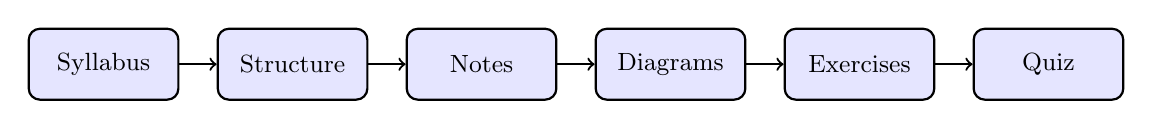
\begin{tikzpicture}[box/.style={draw, rounded corners, thick, fill=blue!10, minimum height=0.9cm, minimum width=1.9cm, align=center, font=\small}]
\node[box] (a) at (0,0) {Syllabus};
\node[box] (b) at (2.4,0) {Structure};
\node[box] (c) at (4.8,0) {Notes};
\node[box] (d) at (7.2,0) {Diagrams};
\node[box] (e) at (9.6,0) {Exercises};
\node[box] (f) at (12.0,0) {Quiz};
\foreach \x/\y in {a/b,b/c,c/d,d/e,e/f} \draw[->, thick] (\x) -- (\y);
\end{tikzpicture}}
\end{center}
\begin{itemize}
\item Each arrow is one CRAFT prompt, and each output gets your review before it moves on.
\item Work one topic fully through the pipeline first, then repeat it for the rest.
\end{itemize}
\end{frame}

%%%%%%%%%%%%%%%%%%%%%%%%%%%%%%%%%%%%%%%%%%%%%%%%%%%
\begin{frame}[fragile]\frametitle{Step 1: Syllabus to Structure}
\begin{itemize}
\item Paste your syllabus and ask for an outline that maps onto sections, subsections and units.
\end{itemize}
\begin{lstlisting}[language=HTML]
You are an experienced Grade 9 science teacher (R).
Here is my syllabus: [PASTE SYLLABUS] (C).
Propose a course outline: 5 sections, each with
3 lessons, each lesson with a one-line goal (A).
Format as a nested list, no extra commentary (T).
\end{lstlisting}
\end{frame}

%%%%%%%%%%%%%%%%%%%%%%%%%%%%%%%%%%%%%%%%%%%%%%%%%%%
\begin{frame}[fragile]\frametitle{Step 2: Expand One Topic with CRAFT}
\begin{itemize}
\item Choose one lesson from the outline and expand it fully before touching the others.
\end{itemize}
\begin{lstlisting}[language=HTML]
You are a patient Grade 9 science teacher (R).
My class knows cells and tissues (C).
Write course notes on photosynthesis: 600 words,
3 headings, 1 worked example, 2 common
mistakes (A). Match the tone of this sample:
[PASTE A PARAGRAPH YOU LIKE] (F).
Simple words, short sentences (T).
\end{lstlisting}
\end{frame}

%%%%%%%%%%%%%%%%%%%%%%%%%%%%%%%%%%%%%%%%%%%%%%%%%%%
\begin{frame}[fragile]\frametitle{Prompts for Course Notes}
\begin{itemize}
\item \textbf{Draft:} ask for notes at a stated level, length and heading structure.
\item \textbf{Adapt:} ask for the same notes at an easier level, or with local examples.
\item \textbf{Shorten:} ask for a one-page cheat sheet from the full notes.
\item \textbf{Check:} ask the AI to list claims in its own notes that you should verify.
\item Save prompts that worked in your prompt library, with placeholders for topic and grade.
\end{itemize}
\end{frame}

%%%%%%%%%%%%%%%%%%%%%%%%%%%%%%%%%%%%%%%%%%%%%%%%%%%
\begin{frame}[fragile]\frametitle{Diagrams as SVG by Prompt}
\begin{itemize}
\item SVG is text, so an AI can write it. It scales cleanly and drops straight into an HTML unit or a slide.
\item Describe the diagram, the labels and the colours; ask for SVG code only.
\end{itemize}
\begin{lstlisting}[language=HTML]
Draw an SVG, 400x200, of a water cycle:
sun top-left, cloud top-right, sea at the
bottom, arrows for evaporation and rain,
each arrow labelled. Output only the SVG code.
\end{lstlisting}
\begin{itemize}
\item Save the reply as \texttt{water\_cycle.svg} and open it in a browser. Ask for fixes in plain words.
\end{itemize}
\end{frame}

%%%%%%%%%%%%%%%%%%%%%%%%%%%%%%%%%%%%%%%%%%%%%%%%%%%
\begin{frame}[fragile]\frametitle{Diagrams: Other Routes}
\begin{itemize}
\item \textbf{Mermaid or Graphviz text:} ask the AI for flowcharts and concept maps as text, then render them.
\item \textbf{draw.io or PowerPoint:} ask for a layout plan and label list, then draw by hand for full control.
\item \textbf{Image generators:} fine for illustrations, but weak at accurate labels; always check the text inside the image.
\item For science and maths diagrams, prefer text-based formats you can inspect and correct.
\end{itemize}
\end{frame}

%%%%%%%%%%%%%%%%%%%%%%%%%%%%%%%%%%%%%%%%%%%%%%%%%%%
\begin{frame}[fragile]\frametitle{Exercises with Graded Difficulty}
\begin{itemize}
\item Ask for exercises in levels, so every student finds a starting point.
\end{itemize}
\begin{lstlisting}[language=HTML]
You are a Grade 9 science teacher (R).
For the photosynthesis notes above (C), write
9 exercises: 3 routine, 3 applied, 3 challenge (A).
Give a short model answer for each (A).
Match the question style of my sample [SAMPLE] (F).
No question may need outside data (T).
\end{lstlisting}
\end{frame}

%%%%%%%%%%%%%%%%%%%%%%%%%%%%%%%%%%%%%%%%%%%%%%%%%%%
\begin{frame}[fragile]\frametitle{Quizzes with Answer Keys}
\begin{itemize}
\item A quiz needs three outputs: the questions, the correct answers, and a short reason for each wrong option.
\end{itemize}
\begin{lstlisting}[language=HTML]
Write 5 multiple-choice questions on
photosynthesis, 4 options each (A).
Return a table: Question | Correct | Why
the correct one is right | Why each wrong
option is wrong (T).
Mix recall and application questions (T).
\end{lstlisting}
\begin{itemize}
\item Keep the answer key in a separate file from the student view, and check each answer yourself.
\end{itemize}
\end{frame}

%%%%%%%%%%%%%%%%%%%%%%%%%%%%%%%%%%%%%%%%%%%%%%%%%%%
\begin{frame}[fragile]\frametitle{A Quiz Item in Open edX Format}
\begin{itemize}
\item Ask the AI to return questions as Open edX problem XML, then paste it into a Problem component in Studio.
\end{itemize}
\begin{lstlisting}[language=HTML]
<problem>
<multiplechoiceresponse>
<label>Which gas do plants take in?</label>
<choicegroup type="MultipleChoice">
<choice correct="false">Oxygen</choice>
<choice correct="true">Carbon dioxide</choice>
<choice correct="false">Nitrogen</choice>
</choicegroup>
</multiplechoiceresponse>
<solution><p>Plants take in carbon
dioxide for photosynthesis.</p></solution>
</problem>
\end{lstlisting}
\end{frame}

%%%%%%%%%%%%%%%%%%%%%%%%%%%%%%%%%%%%%%%%%%%%%%%%%%%
\begin{frame}[fragile]\frametitle{Check Before You Publish}
\begin{itemize}
\item \textbf{Facts:} verify every number, date, name and formula against your textbook.
\item \textbf{Level:} read it as a student would; shorten any sentence you stumble over.
\item \textbf{Diagrams:} check each label and arrow, and test the image on a phone.
\item \textbf{Quiz:} answer every question yourself and confirm the key matches.
\item \textbf{Privacy:} no real student names or data in any prompt sent to a public tool.
\end{itemize}
\end{frame}

\section[Activity]{Workshop Activity}

%%%%%%%%%%%%%%%%%%%%%%%%%%%%%%%%%%%%%%%%%%%%%%%%%%%
\begin{frame}[fragile]\frametitle{Activity: Your Own Course Booklet}
\begin{itemize}
\item Take one syllabus you teach, and build a first booklet in this session.
\item \textbf{Step 1:} write a CRAFT prompt that turns your syllabus into a section and lesson outline.
\item \textbf{Step 2:} pick one lesson and expand it fully with a CRAFT prompt: notes, one diagram, three exercises.
\item \textbf{Step 3:} add a five-question quiz with an answer key.
\item \textbf{Step 4:} review it against the checklist, and swap with a neighbour for comments.
\end{itemize}
\end{frame}

%%%%%%%%%%%%%%%%%%%%%%%%%%%%%%%%%%%%%%%%%%%%%%%%%%%
\begin{frame}[fragile]\frametitle{Flipped Classroom: The Takeaways}
\begin{itemize}
\item Flipping moves content delivery before class and gives class time to discussion and application.
\item Pick the lightest route that works: textbook, notes, playlist or LMS. They combine well.
\item Open edX and Moodle are both free software; the cost is in hosting and set-up, so plan for it.
\item AI drafts structure, notes, diagrams, exercises and quizzes. You decide, correct and own the result.
\end{itemize}
\end{frame}


% \section[Tech]{Optional: For the Technically Curious}
%%%%%%%%%%%%%%%%%%%%%%%%%%%%%%%%%%%%%%%%%%%%%%%%%%%%%%%%%%%%%%%%%%%%%%%%%%%%%%%%%%
\begin{frame}[fragile]\frametitle{}
\begin{center}
{\Large Optional: For the Technically Curious}

\medskip
{\small (Feel free to mentally check out for two slides if this is not your thing, nothing after this needs it.)}
\end{center}
\end{frame}

%%%%%%%%%%%%%%%%%%%%%%%%%%%%%%%%%%%%%%%%%%%%%%%%%%%
\begin{frame}[fragile]\frametitle{The Context Window: Its Working Memory}
\begin{itemize}
\item Everything the model can ``see'' at once, your prompt, any pasted document, the conversation so far, is called the \textbf{context window}.
\item Nothing outside that window exists to the model. It does not remember yesterday's conversation unless you paste it back in.
\item This is exactly why grounding a tool in your school's own documents matters: instead of hoping the model already knows your policy, you retrieve the relevant passage and put it \emph{inside} the context window.
\item Practical rule of thumb: the more relevant material you paste in, the less the model has to guess.
\end{itemize}
\end{frame}

%%%%%%%%%%%%%%%%%%%%%%%%%%%%%%%%%%%%%%%%%%%%%%%%%%%
\begin{frame}[fragile]\frametitle{Why Hallucination Happens}
\begin{itemize}
\item A ``hallucination'' is the model producing a fluent, confident, completely fabricated answer.
\item It happens because the model is optimized to produce \emph{plausible-sounding text}, not to say ``I don't know.''
\item Ask it about a book that does not exist, and it will happily describe the plot.
\item \textbf{Two practical defenses:} give it real source material to work from (same grounding idea as before), and explicitly instruct it to say ``unsure'' when it is not confident.
\end{itemize}
\end{frame}


% ai_educators_wrapup.tex holds 4 sections (Risks/Next/Concl/Refs), folded 2026 from 4 small
% standalone files. See its own header comment for detail.
% Merged 2026: folds ai_educators_risks/_future/_closing/_refs into one file (they were 4
% small standalone files, 9-53 lines each). Section boundaries are marked inline with
% \section so this single \input still produces 4 separate sections in the deck, exactly as
% before the merge.

\section[Risks]{Risks \& Guardrails}

%%%%%%%%%%%%%%%%%%%%%%%%%%%%%%%%%%%%%%%%%%%%%%%%%%%%%%%%%%%%%%%%%%%%%%%%%%%%%%%%%%
\begin{frame}[fragile]\frametitle{}
\begin{center}
{\Large Risks \& Guardrails}
\end{center}
\end{frame}

%%%%%%%%%%%%%%%%%%%%%%%%%%%%%%%%%%%%%%%%%%%%%%%%%%%
\begin{frame}[fragile]\frametitle{Challenges Beyond the Individual Teacher}
\begin{itemize}
\item \textbf{The access gap:} not every student has a phone, a computer, or reliable internet at home. AI-based homework help can quietly widen the gap between students who have access and those who do not, unless the practice stays inside the classroom.
\item \textbf{The literacy gap among staff:} comfort with AI varies a lot teacher to teacher. That gap is itself a challenge to manage, it is exactly what today's talk is meant to help close.
\item \textbf{Cost and choice:} many good tools are free at light use and paid at scale. A school benefits from an agreed, approved list rather than every teacher picking a different tool on their own.
\item These are sector-level challenges. The next few slides cover the risks you manage day to day, in your own use.
\end{itemize}
\end{frame}

%%%%%%%%%%%%%%%%%%%%%%%%%%%%%%%%%%%%%%%%%%%%%%%%%%%
\begin{frame}[fragile]\frametitle{Four Failure Modes Worth Knowing}
\begin{itemize}
\item \textbf{Hallucination:} confidently wrong answers, covered in the AI Basics section, always fact-check anything going to students or parents.
\item \textbf{Academic integrity:} students using AI to write essays undetected. Detection tools are unreliable; redesigning assessments (in-class writing, oral defense, process artifacts) works better than an arms race.
\item \textbf{Over-reliance:} treating the first draft as the final answer, for you or for students. AI output is a starting point, not a verdict.
\item \textbf{Bias:} models trained on internet-scale text inherit internet-scale biases. Review anything touching grading, feedback tone, or student evaluation with that in mind.
\end{itemize}
\end{frame}

%%%%%%%%%%%%%%%%%%%%%%%%%%%%%%%%%%%%%%%%%%%%%%%%%%%
\begin{frame}[fragile]\frametitle{Student Data: The One Non-Negotiable}
\begin{itemize}
\item \textbf{Never paste} student names, grades, health information, or any personally identifiable data into a public, non-institutional AI tool.
\item If your school has an approved, FERPA-compliant (or local equivalent) tool, use that for anything involving real student records.
\item For everything else, anonymize first: ``a Grade 7 student who struggles with fractions'' works just as well as a real name for drafting feedback.
\end{itemize}
\begin{alertblock}{Rule of Thumb}
If you would not write it on a sticky note left on a public desk, do not paste it into a public AI chat window.
\end{alertblock}
\end{frame}

%%%%%%%%%%%%%%%%%%%%%%%%%%%%%%%%%%%%%%%%%%%%%%%%%%%
\begin{frame}[fragile]\frametitle{Quick Check: Spot the Problem}
% [upgrade-deck: rewritten 2026-10-24 | Task 1b | listing must be last, text moved above it]
% \begin{itemize}
% \item A colleague pastes this into a public AI chatbot to get feedback drafted faster:
% \end{itemize}
% \begin{lstlisting}[language=HTML]
% Write encouraging feedback for Priya Sharma, roll no. 23,
% who has been diagnosed with ADHD and is struggling with
% her Grade 8 persuasive essay. Her essay: [pastes full text]
% \end{lstlisting}
% \vspace{15pt}
% \begin{itemize}
% \item What is wrong here, and what is the one-line fix?
% \end{itemize}
\begin{itemize}
\item A colleague pastes this into a public AI chatbot to get feedback drafted faster.
\item What is wrong here, and what is the one-line fix?
\end{itemize}
\begin{lstlisting}[language=HTML]
Write encouraging feedback for Priya Sharma, roll no. 23,
who has been diagnosed with ADHD and is struggling with
her Grade 8 persuasive essay. Her essay: [pastes full text]
\end{lstlisting}
\end{frame}

%%%%%%%%%%%%%%%%%%%%%%%%%%%%%%%%%%%%%%%%%%%%%%%%%%%
\begin{frame}[fragile]\frametitle{Quick Check: Answer}
\begin{itemize}
\item \textbf{The problem:} full name, roll number, and a health diagnosis, all personally identifiable, all sent to a public tool with no institutional data agreement.
\item \textbf{The fix:} drop the name, roll number, and diagnosis. Keep only what the task actually needs: ``a Grade 8 student who needs extra encouragement and structure'' plus the essay text.
\item Same quality of feedback, none of the exposure.
\end{itemize}
\end{frame}

\section[Next]{Where This Goes Next}

%%%%%%%%%%%%%%%%%%%%%%%%%%%%%%%%%%%%%%%%%%%%%%%%%%%%%%%%%%%%%%%%%%%%%%%%%%%%%%%%%%
\begin{frame}[fragile]\frametitle{}
\begin{center}
{\Large Where This Goes Next}
\end{center}
\end{frame}

%%%%%%%%%%%%%%%%%%%%%%%%%%%%%%%%%%%%%%%%%%%%%%%%%%%
\begin{frame}[fragile]\frametitle{From Autocomplete to Agentic Tutors}
\begin{itemize}
\item Today's tools mostly wait for you to ask something, one prompt, one answer.
\item The next wave is \textbf{agentic}: given a goal, the system plans and executes multiple steps on its own, e.g. ``review every submitted exit ticket, flag the three students who need a follow-up, draft a note for each.''
\item Early classroom pilots use this for personalized practice, a system that notices a student is stuck on fractions specifically, not just ``math,'' and adjusts the next problem set accordingly.
\item None of this replaces the teacher's judgment call on \emph{what} to do about it, it just does the noticing faster.
\end{itemize}
\end{frame}

%%%%%%%%%%%%%%%%%%%%%%%%%%%%%%%%%%%%%%%%%%%%%%%%%%%
\begin{frame}[fragile]\frametitle{The Teacher as Orchestrator}
\begin{itemize}
\item New roles are already emerging around this shift, AI-savvy instructional designers, prompt-literate curriculum leads, not just ``teacher'' as a single unchanging job description.
\item The realistic near-term picture is not ``AI teaches, human supervises.'' It is closer to: \textbf{AI handles the repeatable tasks, the teacher spends the reclaimed time on the tasks only a human can do}, noticing, mentoring, adapting in real time.
\item That is the task-vs-job point from earlier, applied forward instead of backward.
\end{itemize}
\end{frame}

\section[Concl]{Closing}

%%%%%%%%%%%%%%%%%%%%%%%%%%%%%%%%%%%%%%%%%%%%%%%%%%%%%%%%%%%%%%%%%%%%%%%%%%%%%%%%%%
\begin{frame}[fragile]\frametitle{}
\begin{center}
{\Large Closing}
\end{center}
\end{frame}

%%%%%%%%%%%%%%%%%%%%%%%%%%%%%%%%%%%%%%%%%%%%%%%%%%%
\begin{frame}[fragile]\frametitle{The One Thing to Remember}
\begin{center}
\Large
\textbf{AI automates tasks.}

\medskip
\textbf{It does not automate jobs.}
\end{center}

\medskip
\begin{itemize}
\item Radiology did not disappear, reading a scan got faster, and the rest of the job stayed human.
\item Teaching will not disappear either. The grading and drafting get faster. The mentoring, the noticing, the trust, that part is still entirely yours.
\item The only real question is which tasks on \emph{your} weekly list are worth handing off this term.
\end{itemize}
\end{frame}

%%%%%%%%%%%%%%%%%%%%%%%%%%%%%%%%%%%%%%%%%%%%%%%%%%%
\begin{frame}[fragile]\frametitle{Start Small: This Week's Action}
\begin{itemize}
\item Pick \textbf{one} recurring task from your own week, a lesson outline, quiz questions, feedback drafts.
\item Write one prompt for it using what you saw in the hands-on section, context, audience, format, constraints.
\item Save the prompt that works. That is the start of your own prompt library, the highest-leverage habit from this whole talk.
\item Next time, you are not starting from a blank page, you are editing a good first draft.
\end{itemize}
\end{frame}

\section[Refs]{References}

%%%%%%%%%%%%%%%%%%%%%%%%%%%%%%%%%%%%%%%%%%%%%%%%%%%%%%%%%%%%%%%%%%%%%%%%%%%%%%%%%%
\begin{frame}\frametitle{References: AI in Education}
\small
\begin{itemize}
\item Fortune, ``A decade after the Godfather of AI said radiologists were obsolete'' (May 2026)
\item Fortune, ``Nvidia CEO Jensen Huang says AI kills tasks not jobs'' (July 2026)
\item New York Times, follow-up interview with Geoffrey Hinton on the 2016 radiology prediction
\item Government of India, YuvaAI / AI for All, FutureSkills Prime
\end{itemize}
\end{frame}

%%%%%%%%%%%%%%%%%%%%%%%%%%%%%%%%%%%%%%%%%%%%%%%%%%%%%%%%%%%%%%%%%%%%%%%%%%%%%%%%%%%
\begin{frame}\frametitle{References}
Many publicly available resources have been refereed for making this presentation. Some of the notable ones are:
\small
\begin{itemize}
\item ``What counts as artificially intelligent? AI and deep learning, explained'' - The Verge
\item ``Artificial Intelligence Overview'' - Harry Surden
\item ``8 ways artificial intelligence is going to change the way you live, work and play in 2018'' - Catherine Clifford
\item ``Artificial intelligence and the future of our work'' - UNDP , IBM Research
\end{itemize}
\end{frame}


\section[Admin]{Appendix: Scaling This at Your Institution}
%%%%%%%%%%%%%%%%%%%%%%%%%%%%%%%%%%%%%%%%%%%%%%%%%%%%%%%%%%%%%%%%%%%%%%%%%%%%%%%%%%
\begin{frame}[fragile]\frametitle{}
\begin{center}
{\Large Appendix: Scaling This at Your Institution}
\end{center}
\end{frame}

%%%%%%%%%%%%%%%%%%%%%%%%%%%%%%%%%%%%%%%%%%%%%%%%%%%%%%%%%%%%%%%%%%%%%%%%%%%%%%%%%%
\begin{frame}[fragile]\frametitle{Three-Tier AI Development Model}
      \begin{itemize}
        \item Progressive pathway: Literacy $\rightarrow$ Proficiency $\rightarrow$ Expertise
        \item Level 1: AI Literacy Drive (AILD) - All faculty
        \item Level 2: AI Proficiency Drive (AIPD) - Builders
        \item Level 3: AI Expertise Drive (AIED) - Researchers
        \item Each level has distinct targets and outcomes
      \end{itemize}
\end{frame}

%%%%%%%%%%%%%%%%%%%%%%%%%%%%%%%%%%%%%%%%%%%%%%%%%%%%%%%%%%%%%%%%%%%%%%%%%%%%%%%%%%
\begin{frame}[fragile]\frametitle{Three-Tier AI Development Model}

      \begin{center}
        \includegraphics[width=0.95\linewidth,keepaspectratio]{AIDrives_banner}
      \end{center}

\end{frame}

% Trimmed from the live "AI for Educators" deck (Aug 2026): this file
% originally opened the seminar as an institutional-rollout pitch (steering
% committee, NAAC accreditation, hackathons). That register fits an admin/
% leadership audience, not a 1-hour talk to classroom teachers, so only the
% Three-Tier Model frames above stay live, repositioned as a closing
% "for administrators" bonus. Everything below is kept on disk, not deleted,
% for possible future re-use (e.g. a dedicated leadership-pitch deck).

% %%%%%%%%%%%%%%%%%%%%%%%%%%%%%%%%%%%%%%%%%%%%%%%%%%%%%%%%%%%%%%%%%%%%%%%%%%%%%%%%%%
% \begin{frame}[fragile]\frametitle{Why Now? The Strategic Imperative}
%   \begin{itemize}
%     \item AI literacy is no longer optional, it is foundational
%     \item Industry expects AI-literate graduates across all branches
%     \item Peer institutions are already implementing AI programs
%     \item Student employability directly linked to AI exposure
%     \item Delayed action creates widening competitive gap
%     \item NAAC accreditation may increasingly evaluate AI readiness
%     \item NEP 2020 emphasizes technology integration across disciplines
%   \end{itemize}
% \end{frame}
%
% %%%%%%%%%%%%%%%%%%%%%%%%%%%%%%%%%%%%%%%%%%%%%%%%%%%%%%%%%%%%%%%%%%%%%%%%%%%%%%%%%%
% \begin{frame}[fragile]\frametitle{Vision and Strategic Approach}
%   \begin{itemize}
%     \item AI for all disciplines, not only CSE/AI branches
%     \item Teacher-first multiplier model: empower faculty to scale impact
%     \item Every teacher uses AI productively and responsibly
%     \item Every department integrates AI where relevant
%     \item Students graduate with practical AI exposure
%     \item Institute becomes recognized AI-enabled ecosystem/campus
%   \end{itemize}
% \end{frame}

% %%%%%%%%%%%%%%%%%%%%%%%%%%%%%%%%%%%%%%%%%%%%%%%%%%%%%%%%%%%%%%%%%%%%%%%%%%%%%%%%%%
% \begin{frame}[fragile]\frametitle{AI Literacy Drive (AILD) - Overview}
  % \begin{itemize}
    % \item Target: All teachers, professors, and administrative staff
    % \item Includes non-technical departments
    % \item Objective: Effective AI tool usage in daily academic workflows
    % \item Expected outcome: Teachers become confident AI users
    % \item Demonstrate AI usage in classroom and academic activities
    % \item Foundation for institute-wide AI adoption
  % \end{itemize}
% \end{frame}

% %%%%%%%%%%%%%%%%%%%%%%%%%%%%%%%%%%%%%%%%%%%%%%%%%%%%%%%%%%%%%%%%%%%%%%%%%%%%%%%%%%
% \begin{frame}[fragile]\frametitle{AILD - Training Topics}
  % \begin{itemize}
    % \item What is AI, Generative AI, and LLMs
    % \item Prompt engineering basics
    % \item AI for lecture prep, notes, question papers, rubrics
    % \item AI for data analysis, reports, presentations
    % % \item Research literature summaries and analysis
    % % \item Responsible AI usage and limitations
    % % \item Copyright, plagiarism awareness, data privacy
    % \item Critical note: Never use confidential institute data in LLMs
  % \end{itemize}
% \end{frame}

% %%%%%%%%%%%%%%%%%%%%%%%%%%%%%%%%%%%%%%%%%%%%%%%%%%%%%%%%%%%%%%%%%%%%%%%%%%%%%%%%%%
% \begin{frame}[fragile]\frametitle{AILD - Delivery Model and Resources}
  % \begin{itemize}
    % \item Online, self-paced, free/low-cost certification (1-2 hours)
    % \item Reputed, preferably non-commercial platforms
    % % \item SOAR AI for Educators (Skill India, requires Aadhar)
    % % \item Swayam-Plus Prompt Engineering (5 hours, free)
    % % \item Great Learning Prompt Engineering (certificate paid)
    % \item YouTube masterclasses as alternatives
    % \item Department-wise awareness recorded or live sessions
    % \item Short hands-on demos, quiz and completion certification
  % \end{itemize}
% \end{frame}

% %%%%%%%%%%%%%%%%%%%%%%%%%%%%%%%%%%%%%%%%%%%%%%%%%%%%%%%%%%%%%%%%%%%%%%%%%%%%%%%%%%
% \begin{frame}[fragile]\frametitle{AILD - Success Metrics}
  % \begin{itemize}
    % \item Percentage of faculty certified
    % \item Percentage of departments participating
    % % \item Number of classroom AI demonstrations
    % % \item Faculty adoption survey results
    % % \item AI literacy certificates issued
    % \item Faculty AI usage examples documented
    % \item Minimum one AI-assisted workflow demo per faculty
  % \end{itemize}
% \end{frame}


% %%%%%%%%%%%%%%%%%%%%%%%%%%%%%%%%%%%%%%%%%%%%%%%%%%%%%%%%%%%%%%%%%%%%%%%%%%%%%%%%%%
% \begin{frame}[fragile]\frametitle{Level 1: AI Literacy Drive (AILD)}
%   \begin{itemize}
%     \item Target: All faculty across all departments
%     \item Delivery: Online self-paced certification (1-2 hours) or Youtube + quiz
%     \item Key capabilities: Prompt engineering, AI-assisted teaching workflows
%     \item Applications: Lecture prep, assessments, research summaries, reports
%     \item Critical principle: Never use confidential data in public LLMs
%     \item Success metrics: 80\% faculty certified, one workflow demo per faculty
%     \item Timeline: Complete baseline certification in 3 months
%     \item Foundation for institution-wide AI adoption
%   \end{itemize}
% \end{frame}

 % %%%%%%%%%%%%%%%%%%%%%%%%%%%%%%%%%%%%%%%%%%%%%%%%%%%%%%%%%%%%%%%%%%%%%%%%%%%%%%%%%%
% \begin{frame}[fragile]\frametitle{AI Proficiency Drive (AIPD) - Overview}
  % \begin{itemize}
    % \item Target: Computer/IT/AI faculty and interested-developer faculty
    % \item Student club teams leads included
    % \item Objective: Build institution-level or Govt AI applications
    % \item Develop domain-specific AI solutions
    % \item Expected outcome: Usable AI systems for academics, participation in hackathons
    % % \item Systems for research and administration
    % \item Move from usage to creation
  % \end{itemize}
% \end{frame}

 % %%%%%%%%%%%%%%%%%%%%%%%%%%%%%%%%%%%%%%%%%%%%%%%%%%%%%%%%%%%%%%%%%%%%%%%%%%%%%%%%%%
% \begin{frame}[fragile]\frametitle{AIPD - Focus Areas}
  % \begin{itemize}
    % \item RAG (Retrieval-Augmented Generation)
    % \item AI chatbots on private institutional data
    % \item Local and private AI deployment
    % \item AI workflow automation and assisted coding
    % \item Agentic AI basics and multimodal AI
    % \item AI APIs and integrations
    % \item Open-source AI ecosystem
  % \end{itemize}
% \end{frame}

% %%%%%%%%%%%%%%%%%%%%%%%%%%%%%%%%%%%%%%%%%%%%%%%%%%%%%%%%%%%%%%%%%%%%%%%%%%%%%%%%%%
% \begin{frame}[fragile]\frametitle{AIPD - Hands-on Projects}
  % \begin{itemize}
    % \item Department-specific chatbots
    % \item Admission query assistant
    % \item Library semantic search system
    % \item Research paper assistant
    % \item Internal knowledge chatbot
    % \item Placement preparation assistant
    % \item Laboratory manual assistant
    % \item Infrastructure: Shared GPU, cloud credits, AI sandbox
  % \end{itemize}
% \end{frame}

% %%%%%%%%%%%%%%%%%%%%%%%%%%%%%%%%%%%%%%%%%%%%%%%%%%%%%%%%%%%%%%%%%%%%%%%%%%%%%%%%%%
% \begin{frame}[fragile]\frametitle{Level 2: AI Proficiency Drive (AIPD)}
%   \begin{itemize}
%     \item Target: Technical faculty and student innovation teams
%     \item Objective: Build institutional AI applications
%     \item Key technologies: RAG systems, chatbots, workflow automation
%     \item Sample projects: Admission assistant, library search, placement tools
%     \item Infrastructure: Shared GPU server, AI sandbox, cloud credits
%     \item Expected outcome: 5-10 deployed AI applications
%     \item Move from usage to creation and problem-solving
%     \item Participation in national AI hackathons and competitions
%   \end{itemize}
% \end{frame}

 % %%%%%%%%%%%%%%%%%%%%%%%%%%%%%%%%%%%%%%%%%%%%%%%%%%%%%%%%%%%%%%%%%%%%%%%%%%%%%%%%%%
% \begin{frame}[fragile]\frametitle{AI Expertise Drive (AIED) - Overview}
  % \begin{itemize}
    % \item Target: AI researchers, PhD scholars, PG students
    % \item Objective: Advanced research capability building
    % \item Build institutional recognition in AI research
    % \item Expected outcome: High-quality research publications
    % \item Funded projects, patents, industry collaborations
    % \item Contribute to cutting-edge AI innovation
  % \end{itemize}
% \end{frame}


 % %%%%%%%%%%%%%%%%%%%%%%%%%%%%%%%%%%%%%%%%%%%%%%%%%%%%%%%%%%%%%%%%%%%%%%%%%%%%%%%%%%
% \begin{frame}[fragile]\frametitle{AIED - Focus Areas and Activities}
  % \begin{itemize}
    % \item Advanced LLMs and domain AI research
    % \item AI for healthcare, manufacturing, agriculture
    % \item Fine-tuning, evaluation, safety, explainability
    % \item Research reading groups and paper mentoring
    % \item Industry problem statements and joint publications
    % \item Targets: Scopus/WoS journals, reputed conferences
    % \item Patents, funded projects, open-source contributions
  % \end{itemize}
% \end{frame}

% %%%%%%%%%%%%%%%%%%%%%%%%%%%%%%%%%%%%%%%%%%%%%%%%%%%%%%%%%%%%%%%%%%%%%%%%%%%%%%%%%%
% \begin{frame}[fragile]\frametitle{Level 3: AI Expertise Drive (AIED)}
%   \begin{itemize}
%     \item Target: Research faculty, PhD scholars, PG students
%     \item Objective: Build institutional research reputation in AI
%     \item Focus: Domain-specific AI (healthcare, manufacturing, agriculture)
%     \item Activities: Research groups, industry collaborations, funded projects
%     \item Expected outcomes: Scopus/WoS publications, patents, grants
%     \item Contribution to cutting-edge AI innovation
%     \item Institutional recognition in national AI research community
%   \end{itemize}
% \end{frame}



 % %%%%%%%%%%%%%%%%%%%%%%%%%%%%%%%%%%%%%%%%%%%%%%%%%%%%%%%%%%%%%%%%%%%%%%%%%%%%%%%%%%
% \begin{frame}[fragile]\frametitle{Driving Committee and Champions}
  % \begin{itemize}
    % \item Steering Committee needed with full ownership of the outcomes
    % \item Define delivery details and  assessment guidelines
    % \item AI Champions Network: 1-2 per department
    % \item Early adopters as mentors and internal trainers
	% \item Pilot with 2-3 colleges/departments
  % \end{itemize}
% \end{frame}

% %%%%%%%%%%%%%%%%%%%%%%%%%%%%%%%%%%%%%%%%%%%%%%%%%%%%%%%%%%%%%%%%%%%%%%%%%%%%%%%%%%
% \begin{frame}[fragile]\frametitle{Governance and Implementation Structure}
%   \begin{itemize}
%     \item Internal AI Steering Committee with full ownership of outcomes
%     % \item Clear policies: usage guidelines, assessment, plagiarism
%     \item AI Champions Network: 1-2 champions per department
%     \item Early adopters serve as mentors and internal trainers
%     \item Pilot approach: Start with 2-3 departments for refinement
%     \item Investment: time of the faculty and fees if any paid certification is selected, else none
%     % \item Continuous upskilling: Quarterly workshops and updates
%   \end{itemize}
% \end{frame}

% %%%%%%%%%%%%%%%%%%%%%%%%%%%%%%%%%%%%%%%%%%%%%%%%%%%%%%%%%%%%%%%%%%%%%%%%%%%%%%%%%%
% \begin{frame}[fragile]\frametitle{Extensions - AI Across All Departments}
  % \begin{itemize}
    % \item AI should not remain limited to CS/IT
    % \item Mechanical: Design calculations, reports
    % \item Civil: Estimation and document analysis
    % \item Finance: Financial analysis and modeling
    % \item Arts: Content creation and research support
    % \item Pharmacy: Literature review and drug research
    % \item Law: Document summarization and case analysis
    % \item Management: Market intelligence and business analytics
  % \end{itemize}
% \end{frame}

% %%%%%%%%%%%%%%%%%%%%%%%%%%%%%%%%%%%%%%%%%%%%%%%%%%%%%%%%%%%%%%%%%%%%%%%%%%%%%%%%%%
% \begin{frame}[fragile]\frametitle{Extensions - Student Engagement}
  % \begin{itemize}
    % \item Faculty training alone is insufficient
    % \item Establish AI clubs and student innovation groups
    % \item AI project exhibitions and demo days
    % \item Internal mini hackathons and competitions
    % \item Convert passive awareness into active building culture
    % \item Student-led initiatives and peer learning
    % \item Bridge classroom learning with hands-on practice
  % \end{itemize}
% \end{frame}

% \begin{frame}[fragile]\frametitle{Extensions - Infrastructure and Upskilling}
  % \begin{itemize}
    % \item Institutional AI Repository for shared resources
    % \item Prompts, teaching examples, lesson plans
    % \item RAG templates, datasets, reusable tools
    % \item Continuous upskilling: Quarterly refresher workshops
    % \item Monthly AI updates and new tools showcase
    % \item Community meetups and internal seminars
    % \item Industry and alumni collaboration for relevance
  % \end{itemize}
% \end{frame}

% %%%%%%%%%%%%%%%%%%%%%%%%%%%%%%%%%%%%%%%%%%%%%%%%%%%%%%%%%%%%%%%%%%%%%%%%%%%%%%%%%%
% \begin{frame}[fragile]\frametitle{Implementation Roadmap}
  % \begin{itemize}
    % \item Phase 1 (0-3 Months): Form AI committee, launch AILD
    % \item Identify AI champions, conduct/suggest awareness sessions
    % \item Complete baseline faculty certification
    % \item Phase 2 (3-6 Months): Launch AIPD workshops
    % \item Create AI lab/sandbox, start faculty-student projects
    % \item Conduct internal hackathon
    % \item Phase 3 (6-12 Months): Launch AIED research clusters
    % \item Publish papers, develop institutional AI tools
    % \item Build industry collaborations
  % \end{itemize}
% \end{frame}


% %%%%%%%%%%%%%%%%%%%%%%%%%%%%%%%%%%%%%%%%%%%%%%%%%%%%%%%%%%%%%%%%%%%%%%%%%%%%%%%%%%
% \begin{frame}[fragile]\frametitle{Implementation Timeline}
%   \begin{itemize}
%     \item Phase 1 (Months 0-3): Foundation
%     \item Form steering committee, identify champions, launch AILD
%     \item Target: 80\% faculty baseline certification
%     \item Phase 2 (Months 3-6): Building
%     \item Launch AIPD workshops, establish AI lab
%     \item Start faculty-student projects, conduct internal hackathon
%     \item Phase 3 (Months 6-12): Excellence
%     \item Launch AIED research clusters, industry partnerships
%     \item Deploy institutional AI tools, publish research papers
%   \end{itemize}
% \end{frame}

% %%%%%%%%%%%%%%%%%%%%%%%%%%%%%%%%%%%%%%%%%%%%%%%%%%%%%%%%%%%%%%%%%%%%%%%%%%%%%%%%%%
% \begin{frame}[fragile]\frametitle{Expected Outcomes and Impact}
%   \begin{itemize}
%     \item Month 3: 80\% faculty AI-certified across all departments
%     \item Month 6: 5+ institutional AI applications deployed
%     \item Month 9: Student AI clubs active, regular hackathons
%     \item Month 12: 2-3 research publications in AI domain
%     \item Improved student placement rates and starting salaries
%     \item Enhanced NAAC scores and institutional rankings
%     \item Recognition as AI-forward institution in state/region
%     % \item Sustainable ecosystem benefiting every future batch
%   \end{itemize}
% \end{frame}

% %%%%%%%%%%%%%%%%%%%%%%%%%%%%%%%%%%%%%%%%%%%%%%%%%%%%%%%%%%%%%%%%%%%%%%%%%%%%%%%%%%
% \begin{frame}[fragile]\frametitle{The Multiplier Effect}
  % \begin{itemize}
    % \item Training 100 students: temporary impact on one batch
    % \item Empowering 50 faculty: permanent impact on 5000+ students
    % \item Teacher-first model creates self-sustaining ecosystem
    % \item Faculty become champions, mentors, and role models
    % \item Natural amplification across every course and semester
    % \item Institutional transformation, not individual training
    % \item The strategic advantage of early adoption compounds over time
  % \end{itemize}
% \end{frame}

% %%%%%%%%%%%%%%%%%%%%%%%%%%%%%%%%%%%%%%%%%%%%%%%%%%%%%%%%%%%%%%%%%%%%%%%%%%%%%%%%%%
% \begin{frame}[fragile]\frametitle{Approval Request and Next Steps}
%   \begin{itemize}
%     \item Approve three-tier AI transformation framework
%     \item Authorize formation of AI Steering Committee
%     \item Approve faculty release time for AI Champions
%     \item Grant autonomy for pilot implementation in 2-3 departments
%     \item Next steps: Committee formation within 2 weeks
%     \item Launch AILD certification drive within 4 weeks
%     \item Time to act is now - competitors are not waiting
%   \end{itemize}
% \end{frame}



% %%%%%%%%%%%%%%%%%%%%%%%%%%%%%%%%%%%%%%%%%%%%%%%%%%%%%%%%%%%%%%%%%%%%%%%%%%%%%%%%%%
% \begin{frame}[fragile]\frametitle{Final Thought}
  % \begin{itemize}
    % \item Teacher-first amplification is the strategic foundation
    % \item Training students gives temporary impact
    % \item Empowering teachers creates long-term ecosystem
    % \item Self-sustaining AI culture emerges
    % \item Every future batch benefits continuously
    % \item Institutional transformation, not individual training
    % \item The multiplier effect is the key to scale
  % \end{itemize}
% \end{frame}

% %%%%%%%%%%%%%%%%%%%%%%%%%%%%%%%%%%%%%%%%%%%%%%%%%%%%%%%%%%%%%%%%%%%%%%%%%%%%%%%%%%
% \begin{frame}[fragile]\frametitle{Summary}
  % \begin{itemize}
    % \item Three-tier framework: Literacy → Proficiency → Expertise
    % \item Teacher empowerment drives sustainable adoption
    % \item All departments included, not just technical
    % \item Governance, champions, and infrastructure essential
    % \item Progressive implementation over 12 months
    % \item Focus on practical outcomes and real applications
    % \item Build an AI-enabled academic ecosystem
  % \end{itemize}
% \end{frame}

